\documentclass[10pt]{article}

\usepackage[margin=0.85in]{geometry}
\usepackage{amsmath}
\usepackage{array}
\usepackage{booktabs}
\usepackage{caption}
\usepackage{graphicx}
\usepackage{hyperref}
\usepackage{microtype}
\usepackage{xcolor}

\graphicspath{{../figures/}{figures/}}

\title{\vspace{-1.0cm}From Text to Torque: Improving RL Tracking of Text-Generated Humanoid Motions}
\author{
Kuzey Kantarcioglu \\
\texttt{kuzey@stanford.edu}
\and
Benji Warburton \\
\texttt{benjiw@stanford.edu}
}
\date{CS224R Final Project}

\begin{document}
\maketitle

\section*{Extended Abstract}

Text-to-motion models can generate plausible humanoid kinematics from natural language, but a visually plausible trajectory is not necessarily dynamically feasible for a torque-controlled robot. This project studies the interface between generated kinematic references and reinforcement-learned physical control. We use KimoLab, which connects Kimodo text-conditioned motion generation to MuJoCo/MuJoCo Warp PPO tracking for the Unitree G1 humanoid. Our main question is which generated reference motions are learnable by downstream PPO tracking, and whether relaxed or curriculum termination settings improve learning on difficult references.

We built a Modal-based experiment pipeline that generates text-conditioned Unitree G1 motions, converts them into MuJoCo reference trajectories, trains PPO tracking policies, periodically saves checkpoints and rollout videos, downloads artifacts, computes reference-motion diagnostics, and produces analysis figures. We evaluate four main prompts: walking forward, waving with the right hand, tapping the head, and squatting down then standing up. We also add a harder jump PPO run and reference-only inspections for roll, backflip, and cartwheel prompts. Before PPO training, we compute simple diagnostics such as root-height range, root speed, and joint acceleration. We then compare loose termination thresholds, strict termination thresholds, abrupt loose-to-strict curricula, a gradual termination-threshold curriculum for squat, and direct calibrated-threshold training.

The main empirical result is that termination design exposes a seed- and path-dependent failure boundary. Strict termination works well for gesture-like motions: wave and tap-head policies reach near-full episode lengths and final rewards around 18 under strict thresholds. Walking is also learnable under strict termination, reaching final reward 13.12 and mean episode length 244.78 out of 250. In contrast, strict termination fails severely on one squat reference seed, which has the largest root-height range among our initial references. The loose seed-0 squat policy reaches final reward 13.66 and full 250-step episodes, while the strict seed-0 squat policy reaches only reward 0.84 and terminates after 13.52 steps on average. A second squat seed later shows that strict training can recover with enough samples, but loose termination is more robust early and across seeds.

The curriculum experiments are useful negative results, but they are more informative after adding a gradual schedule. Our two-stage walk curriculum successfully resumes training from a loose first stage into a strict second stage, but it does not outperform strict training from scratch. On squat seed 0, abrupt loose-to-strict transfer collapses back to short episodes. A gradual schedule survives thresholds of 20, 10, 5, and 2, mostly survives threshold 1, and then collapses under the default strict thresholds. This localizes the failure boundary rather than simply showing that curriculum code failed. We then use this boundary to train new squat policies from scratch with fixed calibrated thresholds. Direct threshold-2 training reaches full episodes, reward 12.41, and zero final terminations; direct threshold-1 training also mostly recovers, reaching reward 9.21 and 241.82-step episodes. The jump loose-termination run reaches full episodes with final reward 15.63, showing that semantic difficulty alone is not enough to predict failure. Overall, the project provides a small but complete empirical study of the gap between text-generated kinematic motion and physically executable humanoid control, plus a concrete calibrated-termination intervention for the hardest seed-0 squat case.

\clearpage

\section*{Main Paper}

\section{Introduction}

Language-conditioned robotics systems ultimately need to translate high-level text commands into physically stable low-level behavior. Recent text-to-motion models make the first part of this pipeline increasingly practical: given prompts such as ``walk forward'' or ``squat down and stand up,'' they can synthesize full-body humanoid motion trajectories. However, these trajectories are usually kinematic. They may ignore torque limits, contact timing, balance, self-collisions, and the fact that a controller must recover from tracking error in simulation.

This project studies the gap between generated kinematic motion and reinforcement-learned humanoid control. We use KimoLab as an end-to-end testbed: Kimodo generates Unitree G1 reference motions from text, KimoLab converts them into MuJoCo reference trajectories, and PPO trains policies to track those references. Rather than treating the pipeline as only a demo, we ask when and why the tracking stage succeeds or fails.

Our main research question is:
\begin{quote}
Which properties of a text-generated reference motion determine whether PPO can learn a stable tracking policy, and can relaxed or curriculum termination settings improve learning on difficult generated motions?
\end{quote}

We focus on a practical empirical result rather than state-of-the-art performance. The core contribution is a small but complete study of the failure boundary between text-generated reference motions and dynamically feasible humanoid tracking.

\section{Related Work}

Our project builds on text-conditioned motion generation, physics-based motion imitation, and reinforcement learning for humanoid control. Kimodo is a recent controllable kinematic motion generation system that supports natural-language generation for multiple skeletons, including the Unitree G1 humanoid robot \cite{kimodo,kimodo_github}. KimoLab connects Kimodo-generated motions to MuJoCo/MuJoCo Warp tracking experiments \cite{kimolab,mujoco,mujocowarp}. This makes it useful for studying text-to-physics pipelines with real robot morphologies.

Physics-based character imitation methods such as DeepMimic show that deep RL can learn agile simulated behaviors from reference motion clips \cite{deepmimic}. Adversarial Motion Priors extend this idea by learning a motion prior from datasets, reducing reliance on hand-designed imitation rewards \cite{amp}. These methods typically assume curated or motion-capture reference data. In contrast, our references are generated automatically from text and may contain artifacts that make downstream tracking harder.

We use PPO as the tracking optimizer, following its broad use in continuous-control RL and robotics \cite{ppo}. Our focus is not on changing PPO itself, but on understanding how generated reference quality and episode termination interact with PPO learning.

\section{Method}

\subsection{Pipeline}

The experimental pipeline is:
\[
\text{text prompt} \rightarrow \text{Kimodo CSV motion} \rightarrow \text{MuJoCo NPZ reference} \rightarrow \text{PPO tracking policy}.
\]

All final experiments used 4 second motions, resampled to 50 Hz, with PPO training in MuJoCo Warp on Modal GPUs. Training used 1024 parallel environments and 2000 PPO iterations unless otherwise noted. Each policy was trained to track the generated reference motion for the Unitree G1 humanoid.

\subsection{Reference-Motion Diagnostics}

Before training, we compute simple diagnostics from the generated reference trajectories:
\begin{itemize}
    \item root height range,
    \item maximum root speed,
    \item maximum root acceleration,
    \item maximum joint velocity and acceleration,
    \item rollout artifact counts, including checkpoints and videos.
\end{itemize}

These diagnostics are intentionally simple. They are meant to test whether cheap pre-training measurements can identify references that are likely to be difficult for PPO tracking.

\subsection{Termination Conditions}

We compare five termination settings:
\begin{itemize}
    \item \textbf{Loose}: large tracking-deviation thresholds, so the policy can experience the full reference even when tracking is poor early in training.
    \item \textbf{Strict}: standard tighter tracking-deviation thresholds, so episodes end when the robot deviates too far from the reference.
    \item \textbf{Curriculum}: a two-stage schedule used for walking and squat: 1000 iterations with loose thresholds, then resume from that checkpoint for 1000 iterations with strict thresholds.
    \item \textbf{Gradual curriculum}: a seven-stage squat schedule with thresholds $100, 20, 10, 5, 2, 1$, then strict defaults, used to test where loose tracking becomes brittle.
    \item \textbf{Calibrated threshold}: fixed intermediate termination thresholds chosen from the gradual curriculum boundary, then trained from scratch on the same generated squat reference.
\end{itemize}

The motivation is that strict termination can be useful once a policy is competent, but harmful if it ends episodes before the policy observes enough of the motion to improve.

\section{Experiments}

We evaluate four prompts:
\begin{center}
\begin{tabular}{lll}
\toprule
Motion & Prompt & Main role \\
\midrule
Walk & A person walks forward & Locomotion baseline \\
Wave & A person waves with their right hand & Easy upper-body gesture \\
Tap head & A person taps themselves on the head & Easy upper-body gesture \\
Squat & A person squats down and stands up & Large root-height change \\
\bottomrule
\end{tabular}
\end{center}

The main quantitative metrics are final reward, mean episode length, body-position tracking error, joint-position tracking error, and termination counts. We also save training videos and checkpoints throughout training. Episode length is crucial when comparing termination settings, because low tracking error over very short episodes can be misleading.

After the main training runs, we also generated harder prompts: jump, roll forward, backflip, and cartwheel. We trained jump with loose termination and used roll, backflip, and cartwheel as reference-only qualitative feasibility checks.

\section{Results}

\subsection{Reference Diagnostics}

Figure~\ref{fig:diagnostics} shows the pre-training diagnostics. The prompts differ in intuitive ways: squat has the largest root-height range, walk has the highest root speed, and wave has high joint acceleration despite being easy to track. This means that high joint acceleration alone is not sufficient to predict failure. In this suite, large vertical/root motion combined with strict termination is a stronger warning sign.

\begin{figure}[t]
    \centering
    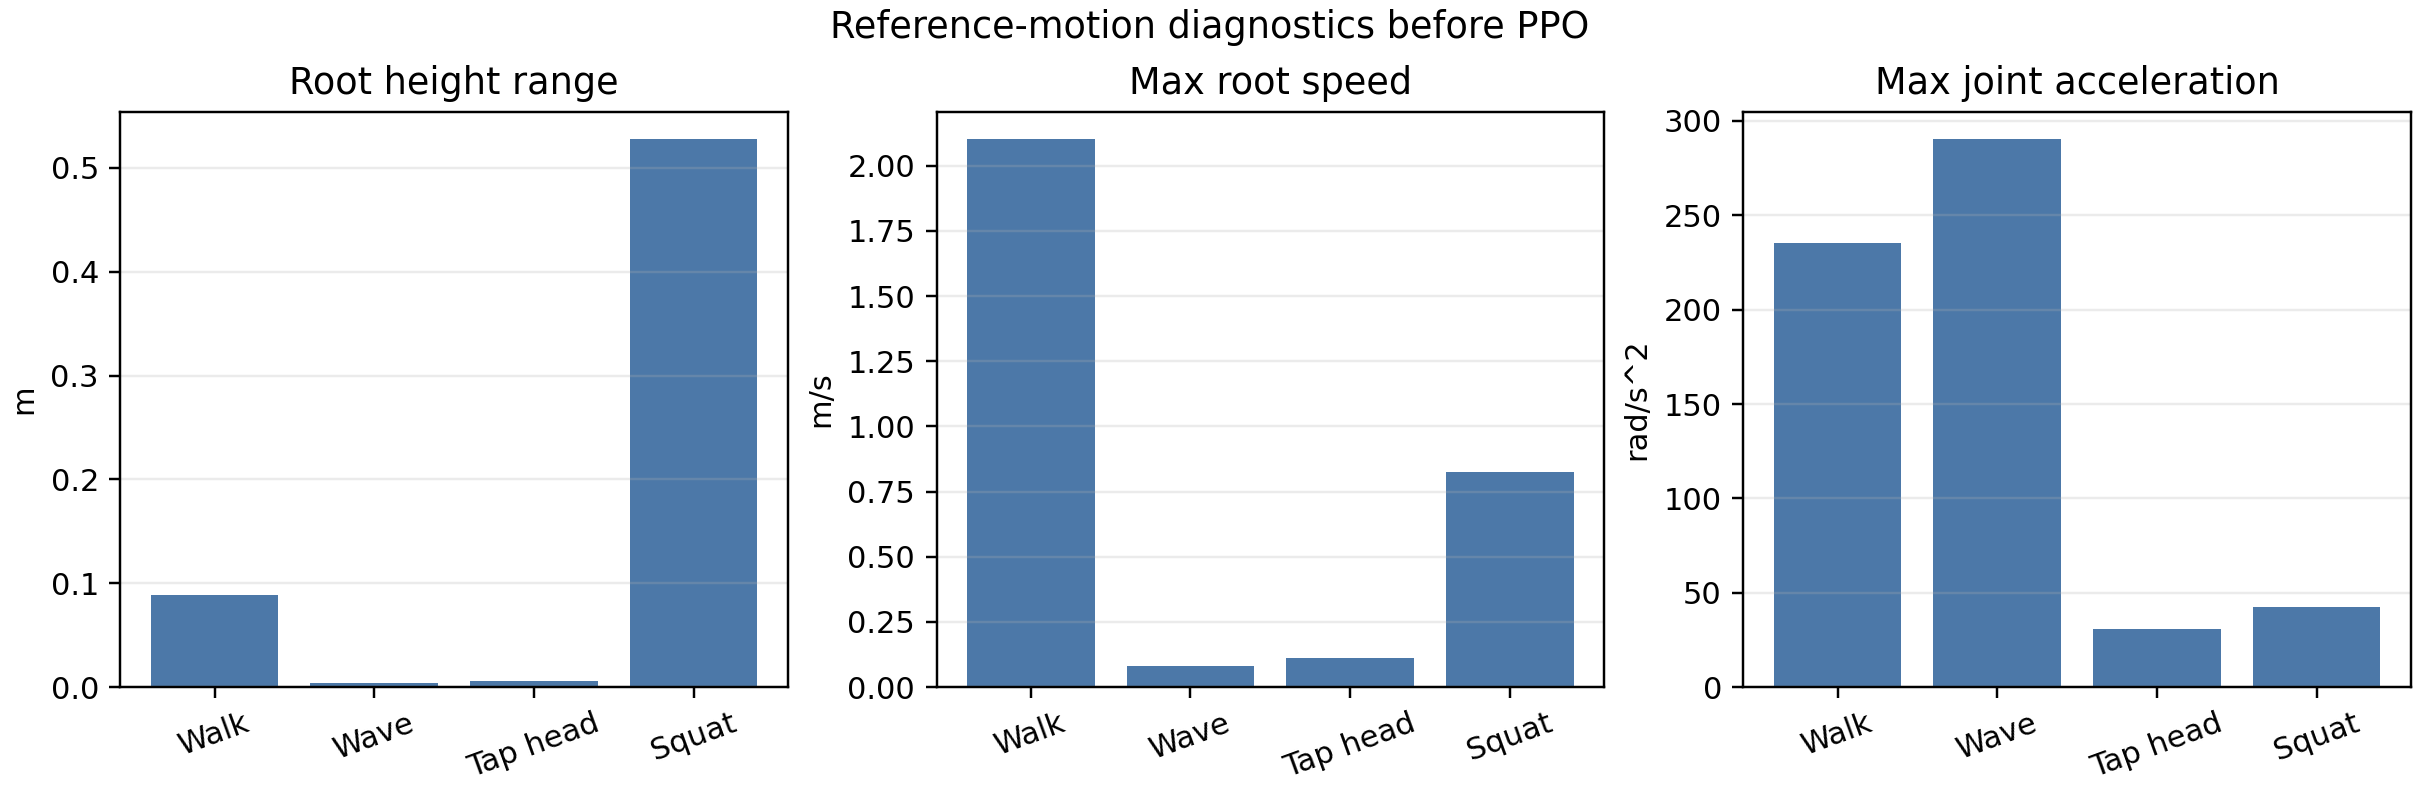
\includegraphics[width=\linewidth]{final_reference_diagnostics.png}
    \caption{Reference-motion diagnostics before PPO training. Squat has the largest root-height range, while walk has the highest root speed.}
    \label{fig:diagnostics}
\end{figure}

\subsection{Final Tracking Outcomes}

Table~\ref{tab:summary} summarizes the final outcomes. Gesture-like motions are robust to strict termination: wave and tap head reach near-full episode length under both loose and strict settings. Walk also remains learnable under strict termination. The clearest failure occurs for squat under strict termination. The loose squat policy reaches the full 250-step horizon, while the strict squat policy averages only 13.52 steps and accumulates a large termination count.

\begin{table}[t]
\centering
\caption{Final PPO tracking outcomes. Termination total is the sum of anchor-position and end-effector/body-position terminations reported at the end of training.}
\label{tab:summary}
\resizebox{\linewidth}{!}{
\begin{tabular}{llrrrrr}
\toprule
Motion & Condition & Reward & Episode length & Body pos. err. & Joint pos. err. & Term. total \\
\midrule
Walk & Loose & 11.352 & 250.00 & 0.123 & 0.916 & 0.000 \\
Walk & Strict & 13.123 & 244.78 & 0.075 & 0.832 & 0.333 \\
Walk & Curriculum & 11.186 & 232.64 & 0.089 & 0.905 & 0.500 \\
Wave & Loose & 18.132 & 250.00 & 0.035 & 0.622 & 0.000 \\
Wave & Strict & 18.068 & 250.00 & 0.036 & 0.606 & 0.000 \\
Tap head & Loose & 18.450 & 250.00 & 0.045 & 0.575 & 0.000 \\
Tap head & Strict & 17.409 & 246.68 & 0.041 & 0.650 & 0.083 \\
Squat & Loose & 13.657 & 250.00 & 0.271 & 1.545 & 0.000 \\
Squat & Strict & 0.837 & 13.52 & 0.234 & 0.484 & 144.875 \\
\bottomrule
\end{tabular}}
\end{table}

Figure~\ref{fig:outcomes} visualizes the same result. The strict squat run is the outlier: low reward, very short episodes, and many terminations. The strict squat body/joint error is lower than loose in Table~\ref{tab:summary}, but this is not evidence of better tracking because the policy terminates almost immediately and only evaluates a small early segment of the reference.

\begin{figure}[t]
    \centering
    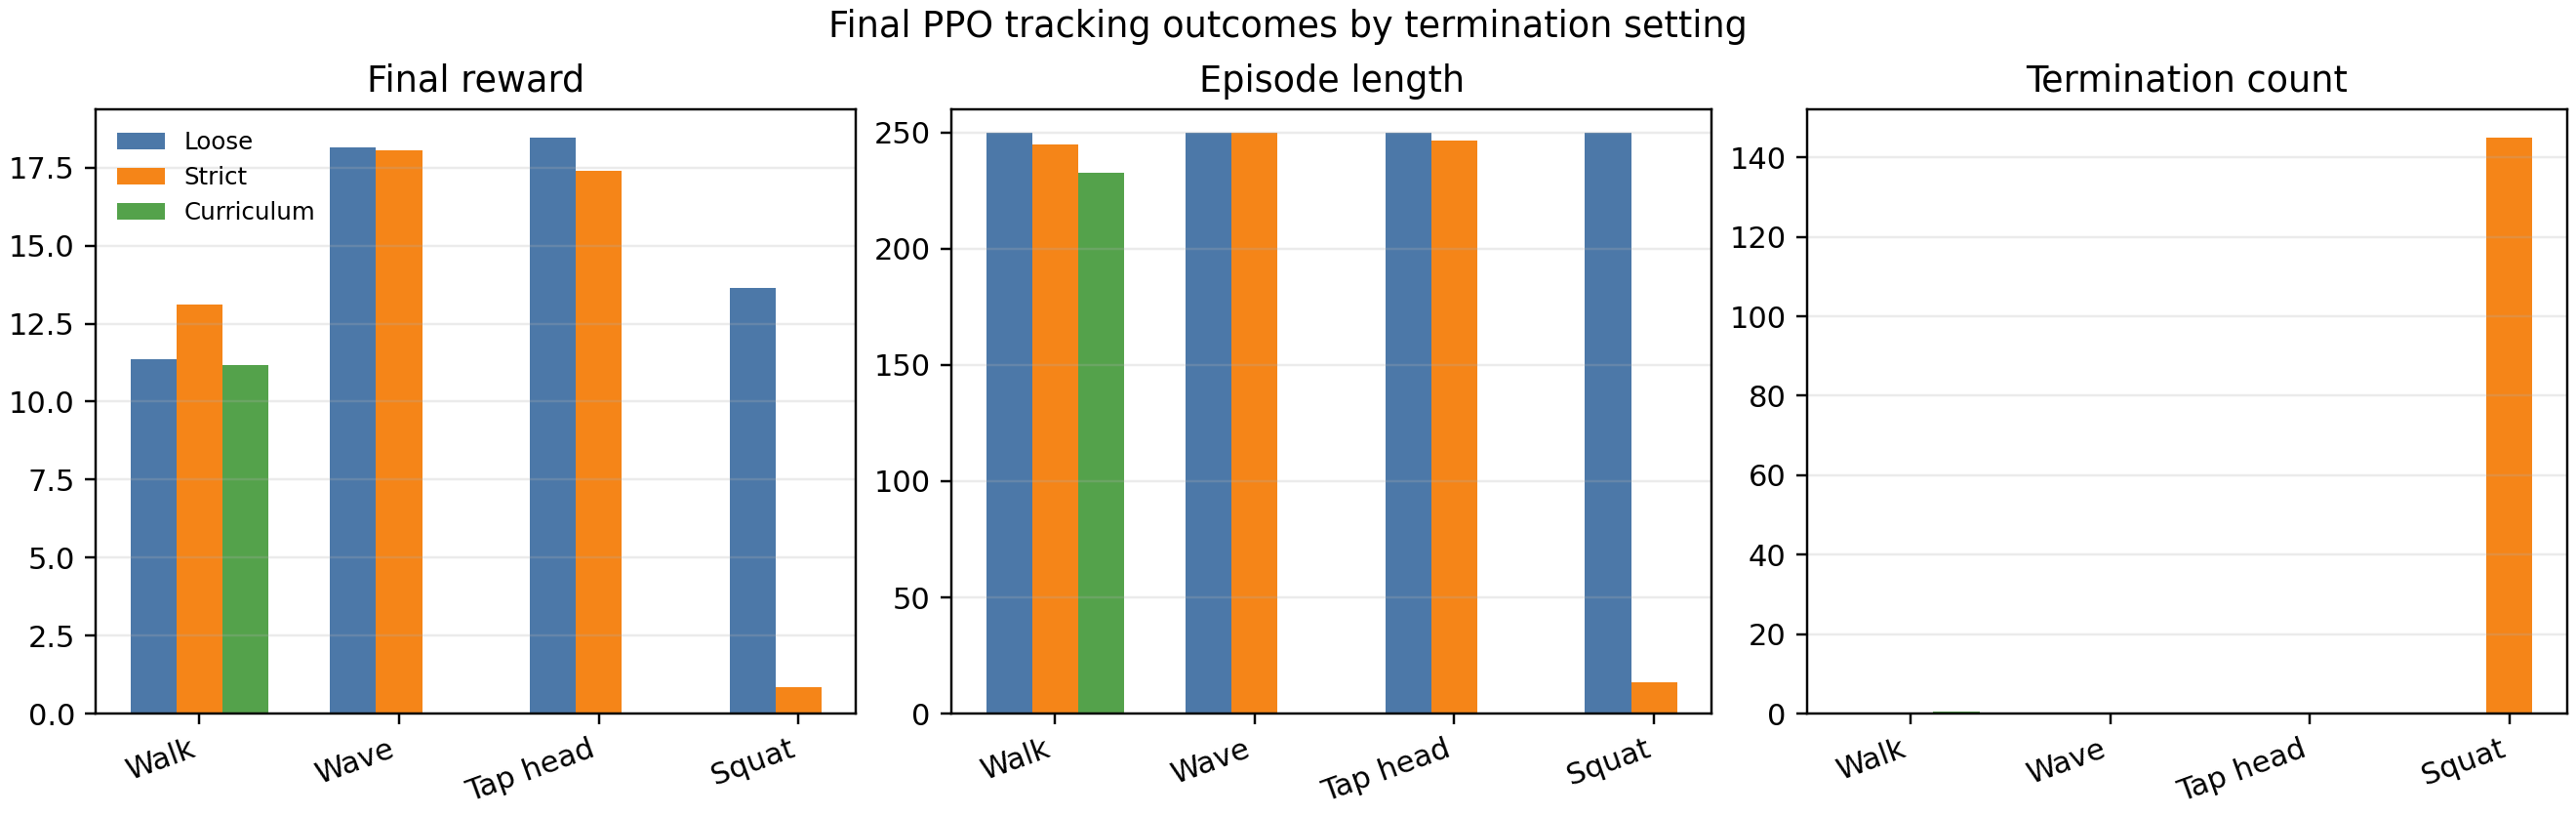
\includegraphics[width=\linewidth]{final_outcome_summary.png}
    \caption{Final outcomes by motion and termination setting. Strict termination fails on squat, while gesture motions remain stable.}
    \label{fig:outcomes}
\end{figure}

\subsection{Squat: Strict Termination Blocks Full-Horizon Learning}

Figure~\ref{fig:squat_curves} shows the learning curves for squat. Loose termination quickly reaches the full horizon and steadily improves reward. Strict termination remains near zero reward and near-zero episode length. This supports the hypothesis that strict termination can prevent exploration and learning for difficult generated motions.

\begin{figure}[t]
    \centering
    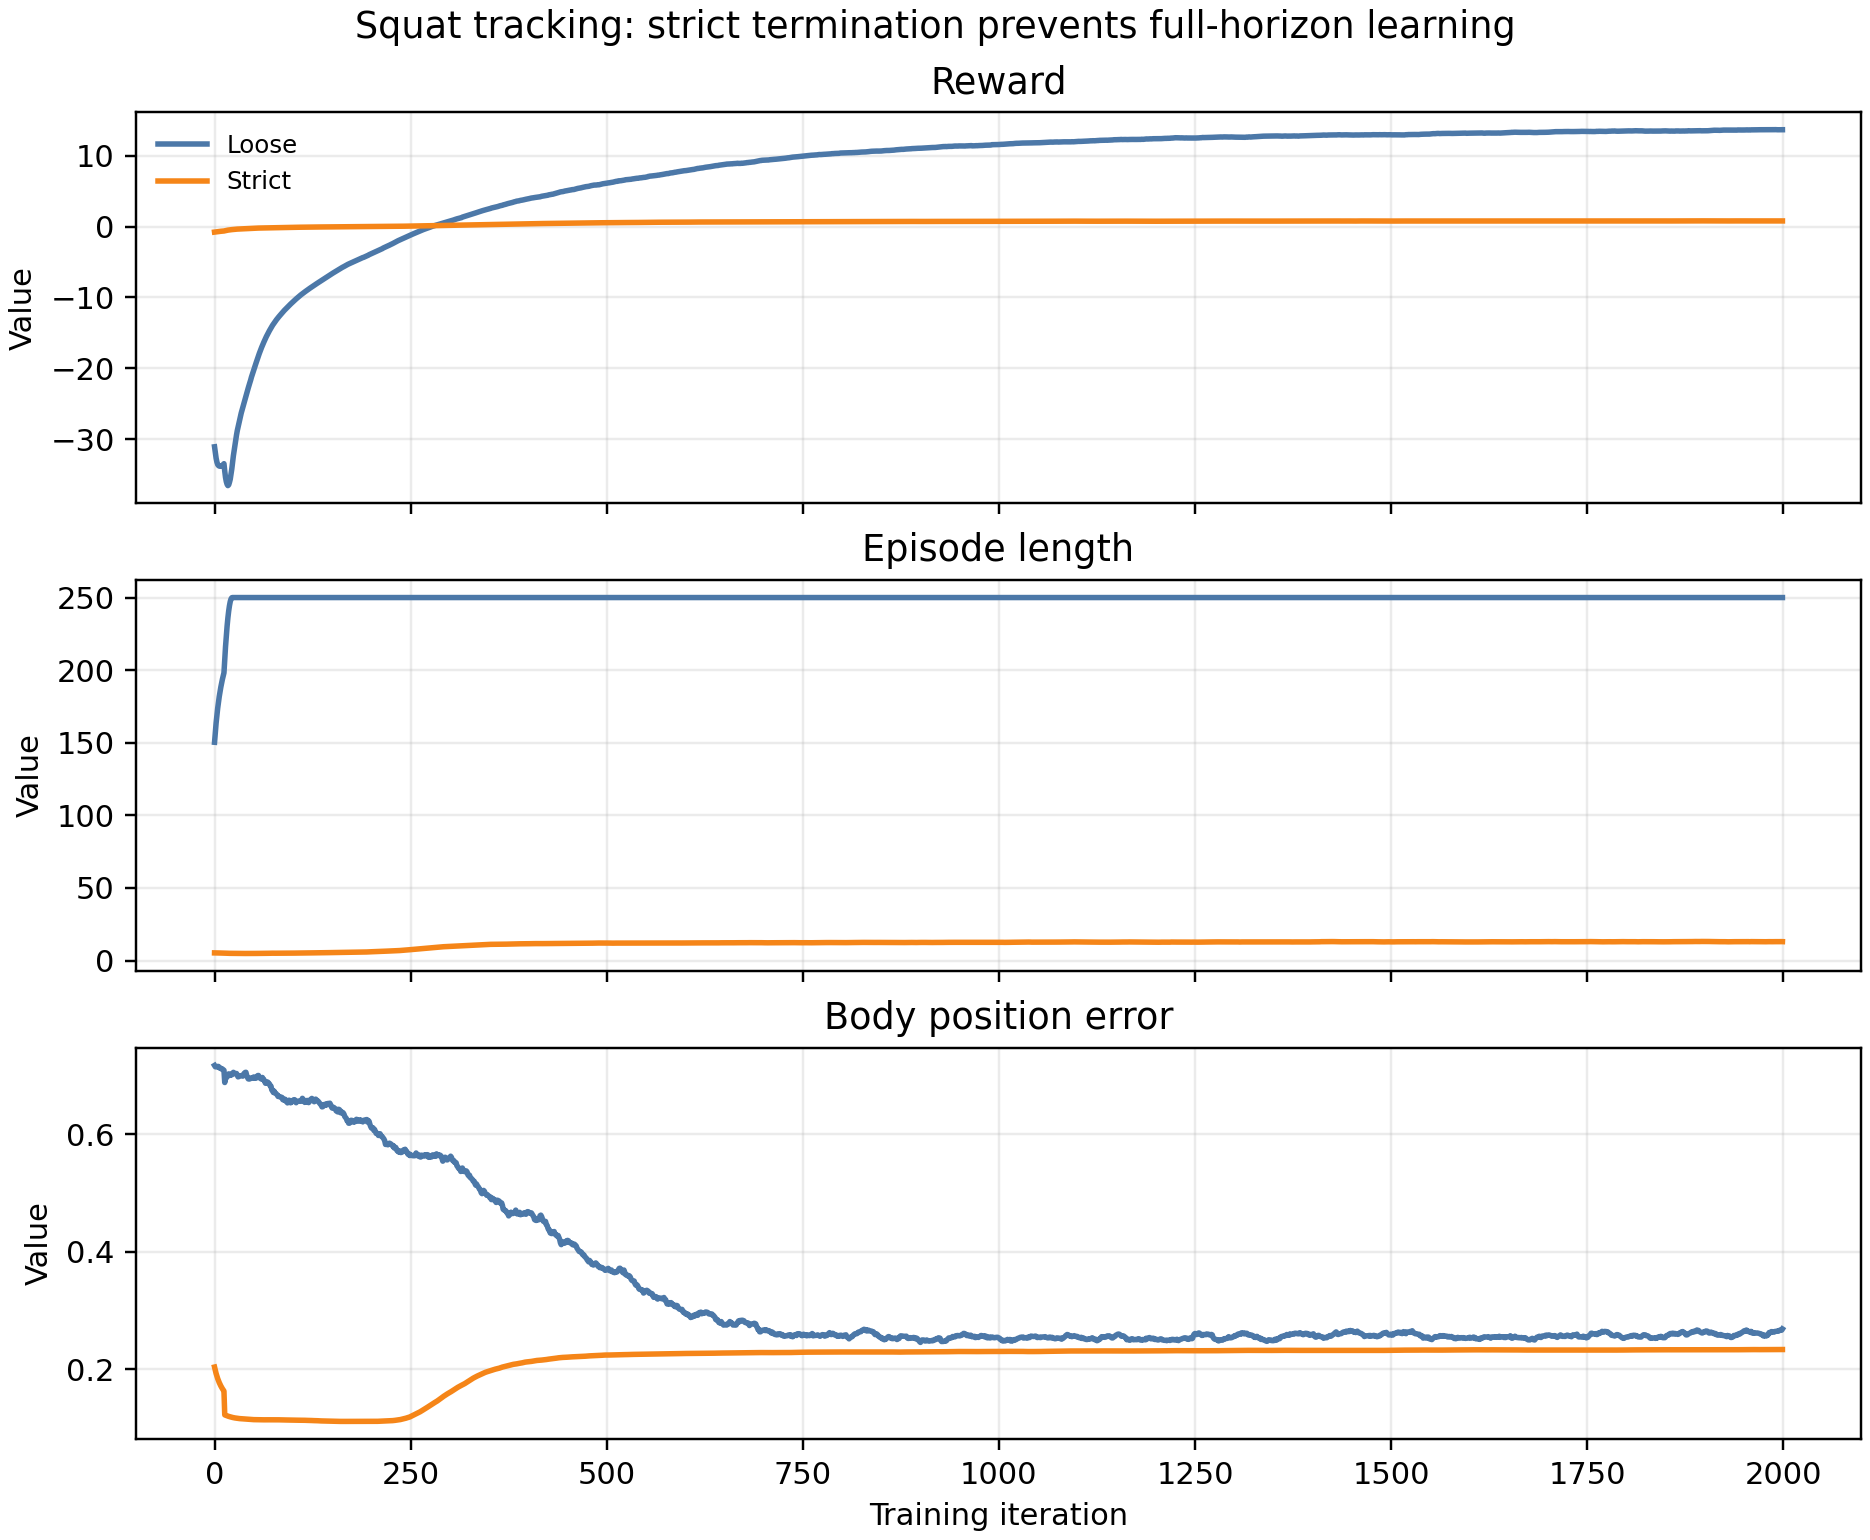
\includegraphics[width=\linewidth]{final_squat_termination_curves.png}
    \caption{Squat learning curves. Loose termination enables full-horizon training, while strict termination repeatedly ends the episode early.}
    \label{fig:squat_curves}
\end{figure}

\subsection{Walk Curriculum}

Figure~\ref{fig:walk_curves} compares loose, strict, and curriculum training for walk. The curriculum run successfully resumes from a loose stage into a strict stage, but it does not outperform strict training from scratch on final reward or episode length. This is an important negative result: relaxing terminations helps clearly on squat, but the simple curriculum we tested is not automatically better on easier locomotion.

\begin{figure}[t]
    \centering
    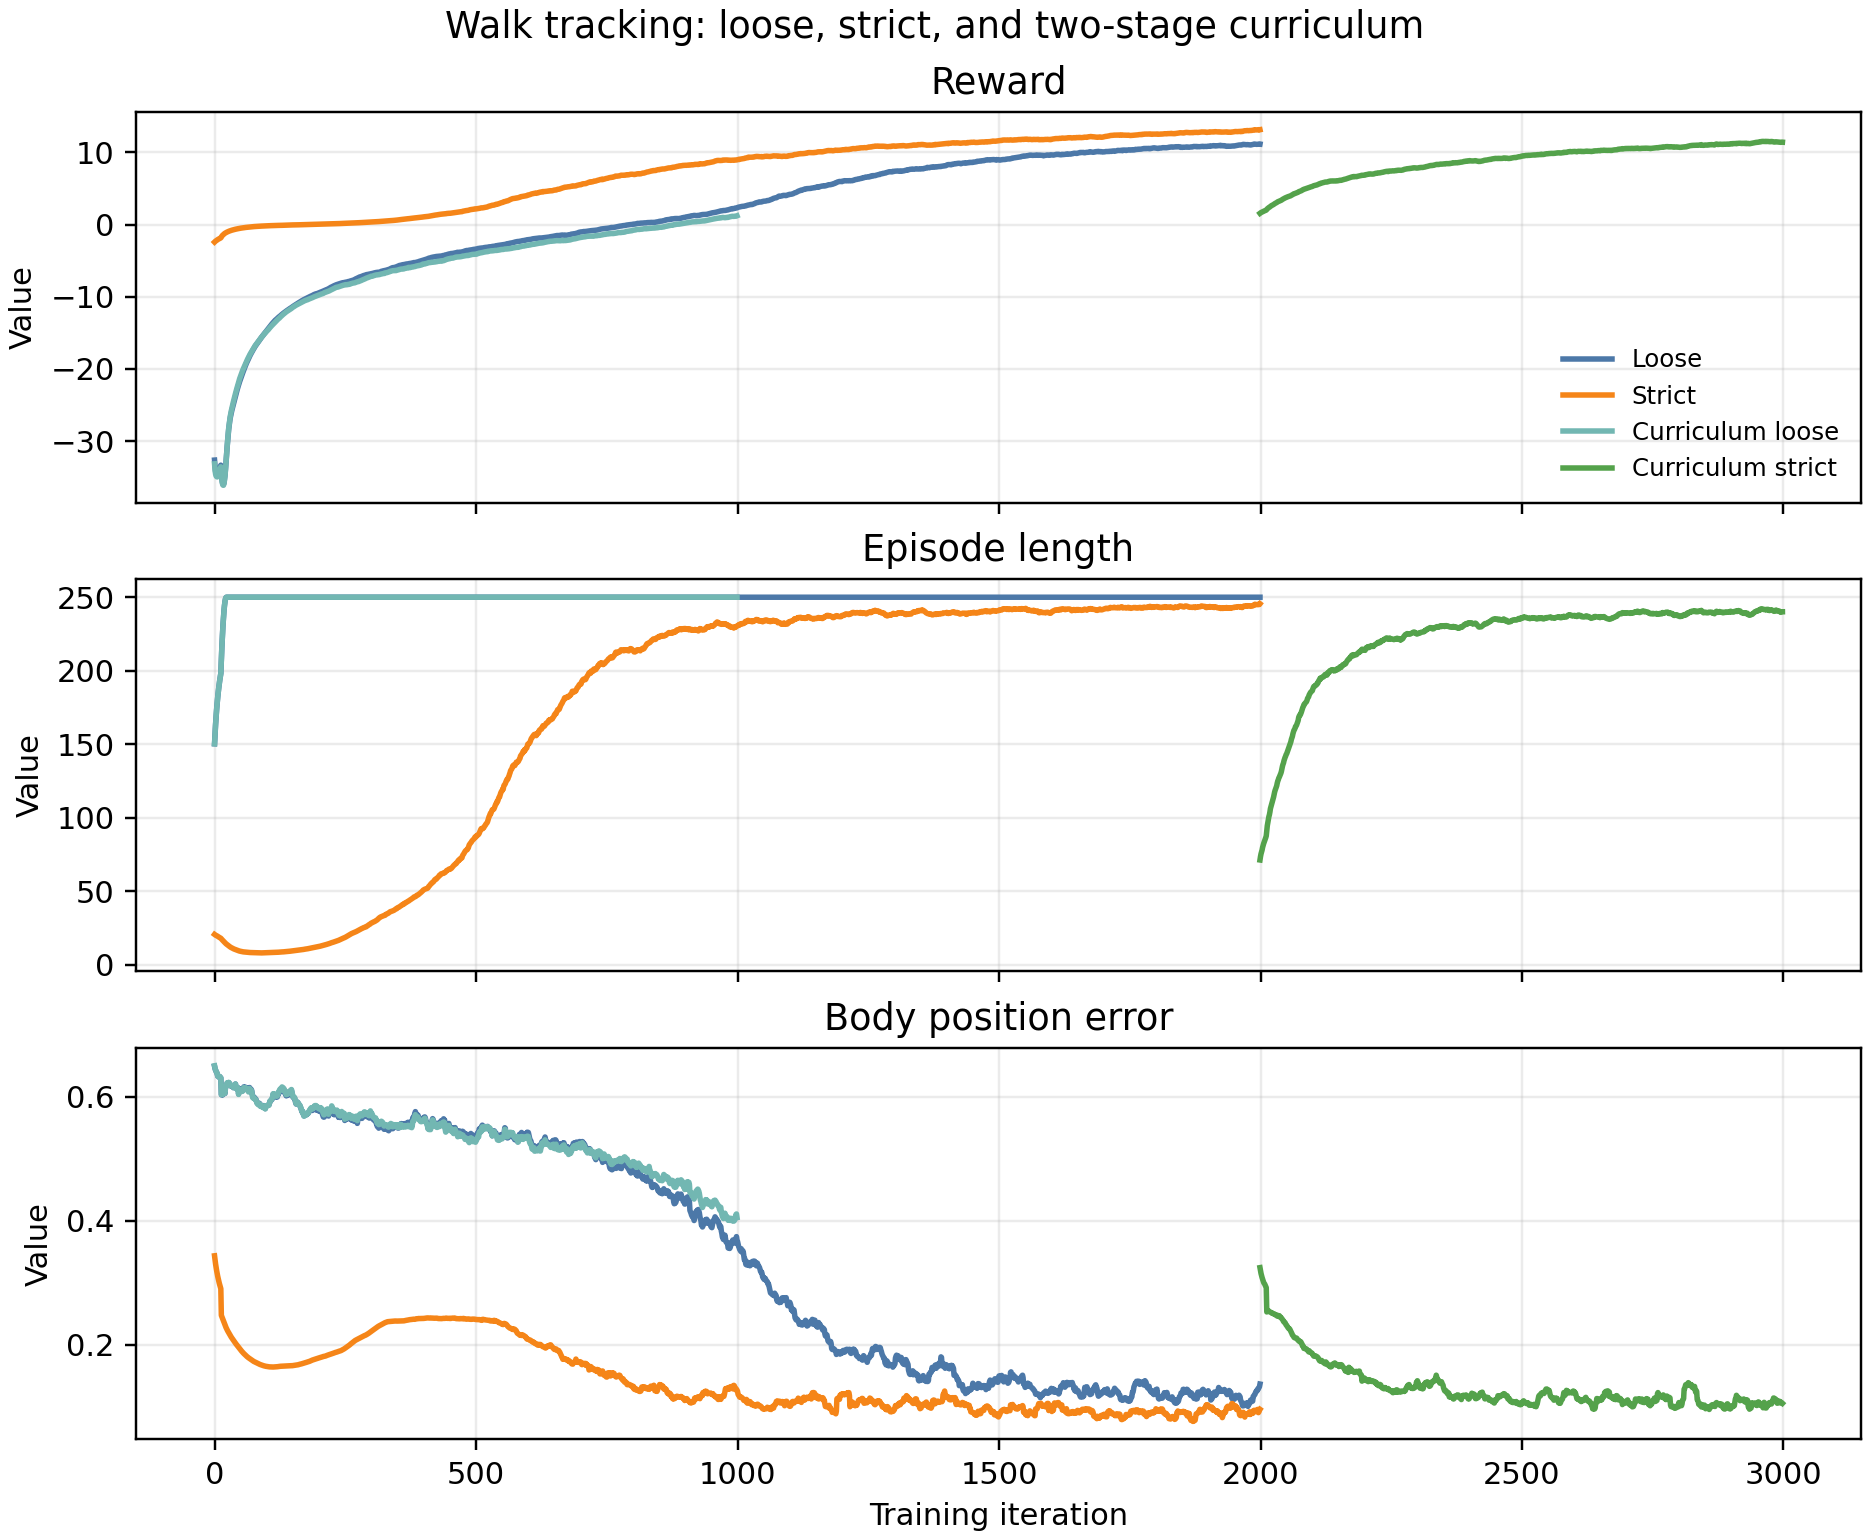
\includegraphics[width=\linewidth]{final_walk_curriculum_curves.png}
    \caption{Walk learning curves. The two-stage curriculum runs successfully, but strict training from scratch performs best in this setting.}
    \label{fig:walk_curves}
\end{figure}

\subsection{Additional Squat Replication and Curriculum Test}

We ran additional squat experiments because the initial seed-0 squat result was the clearest failure case. Table~\ref{tab:extra_squat} and Figure~\ref{fig:extra_squat} show that the result is seed- and training-path dependent. Loose termination is robust across both squat seeds. Strict termination fails badly for seed 0 in the initial experiment, but strict training on seed 1 eventually reaches near-full episodes by 2000 iterations. The seed-0 squat curriculum is a negative result: the loose first stage reaches full-horizon behavior, but switching abruptly to strict thresholds collapses to 12.61-step episodes.

\begin{table}[t]
\centering
\caption{Additional squat experiments. The seed-0 curriculum succeeds during the loose stage but collapses after strict transfer; seed-1 strict training eventually recovers.}
\label{tab:extra_squat}
\resizebox{\linewidth}{!}{
\begin{tabular}{lrrrrr}
\toprule
Condition & Reward & Episode length & Body pos. err. & Joint pos. err. & Term. total \\
\midrule
Seed 0 curriculum, loose stage & 11.619 & 250.00 & 0.249 & 1.848 & 0.000 \\
Seed 0 curriculum, strict stage & 0.772 & 12.61 & 0.230 & 0.436 & 144.333 \\
Seed 1 loose & 12.698 & 250.00 & 0.096 & 1.146 & 0.000 \\
Seed 1 strict & 13.963 & 246.82 & 0.054 & 0.890 & 0.167 \\
\bottomrule
\end{tabular}}
\end{table}

\begin{figure}[t]
    \centering
    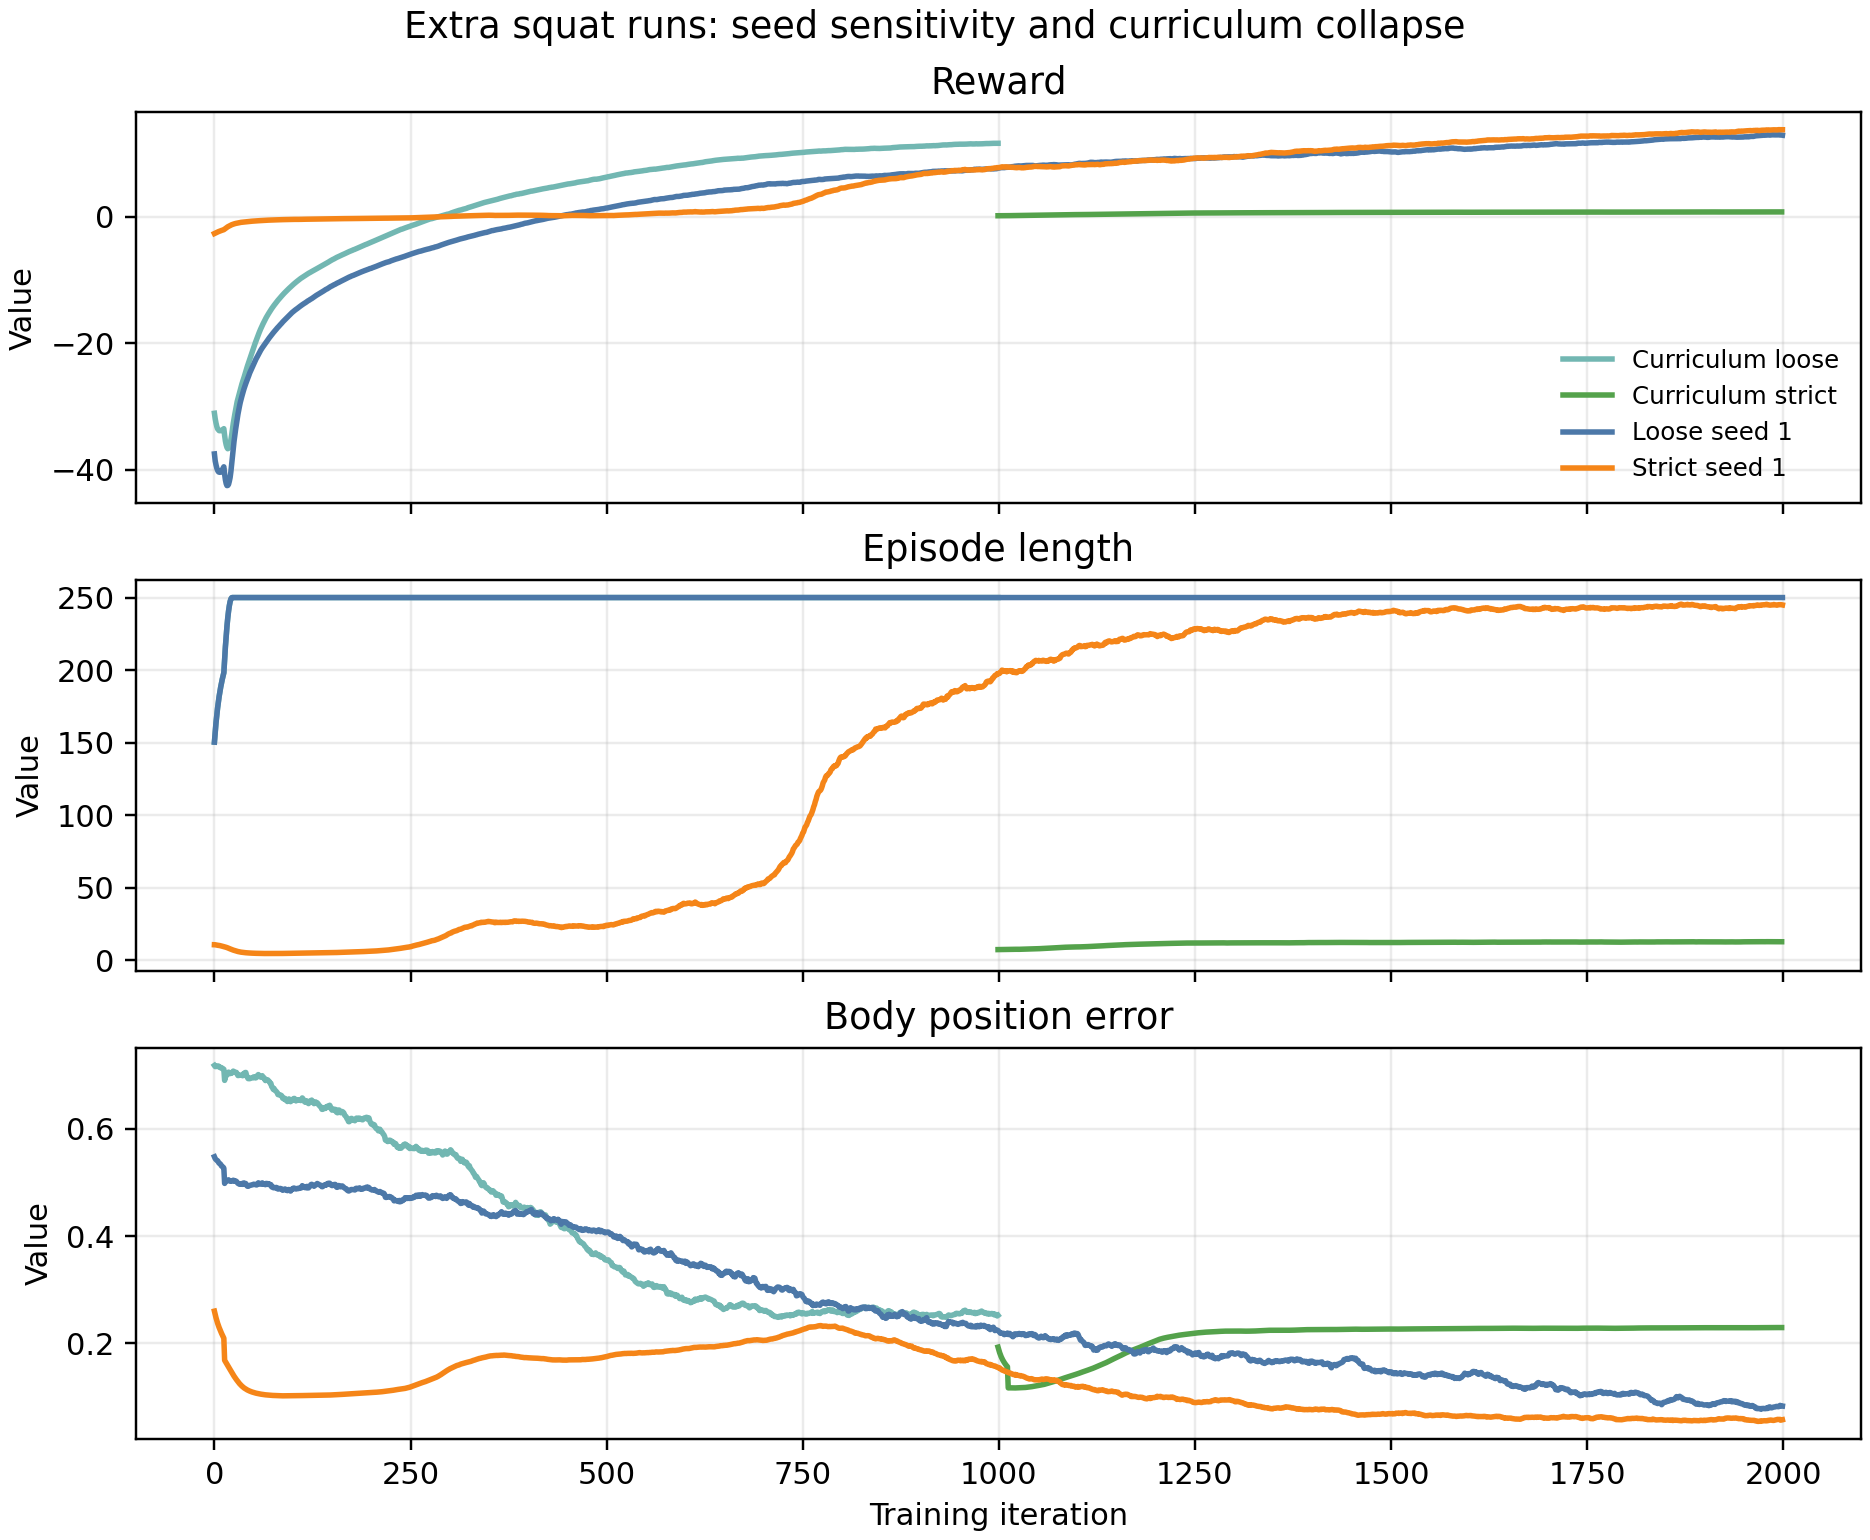
\includegraphics[width=\linewidth]{final_squat_extra_curves.png}
    \caption{Additional squat learning curves. Strict seed 1 eventually recovers, but the seed-0 loose-to-strict curriculum collapses under strict thresholds.}
    \label{fig:extra_squat}
\end{figure}

\subsection{Gradual Squat Curriculum}

Because the abrupt seed-0 squat curriculum failed, we added a more gradual termination schedule: loose threshold 100, then 20, 10, 5, 2, 1, and finally the default strict thresholds. Table~\ref{tab:gradual_squat} and Figure~\ref{fig:gradual_squat} show that the policy remains full-horizon through threshold 2 and mostly full-horizon at threshold 1. The final strict stage still collapses to 12.33-step episodes. This is a stronger diagnostic result than the abrupt curriculum alone: the seed-0 squat policy is not simply unable to improve after loose training, but it is unable to satisfy the final strict termination rule.

\begin{table}[t]
\centering
\caption{Gradual seed-0 squat curriculum. The policy survives intermediate thresholds but collapses under the default strict termination thresholds.}
\label{tab:gradual_squat}
\resizebox{\linewidth}{!}{
\begin{tabular}{lrrrrr}
\toprule
Stage & Reward & Episode length & Body pos. err. & Joint pos. err. & Term. total \\
\midrule
Threshold 100 & 4.510 & 250.00 & 0.554 & 2.504 & 0.000 \\
Threshold 20 & 10.724 & 250.00 & 0.293 & 1.752 & 0.000 \\
Threshold 10 & 12.386 & 250.00 & 0.283 & 1.656 & 0.000 \\
Threshold 5 & 13.108 & 250.00 & 0.287 & 1.489 & 0.000 \\
Threshold 2 & 13.040 & 250.00 & 0.293 & 1.708 & 0.000 \\
Threshold 1 & 11.934 & 244.86 & 0.294 & 1.423 & 0.083 \\
Strict & 0.707 & 12.33 & 0.227 & 0.484 & 145.667 \\
\bottomrule
\end{tabular}}
\end{table}

\begin{figure}[t]
    \centering
    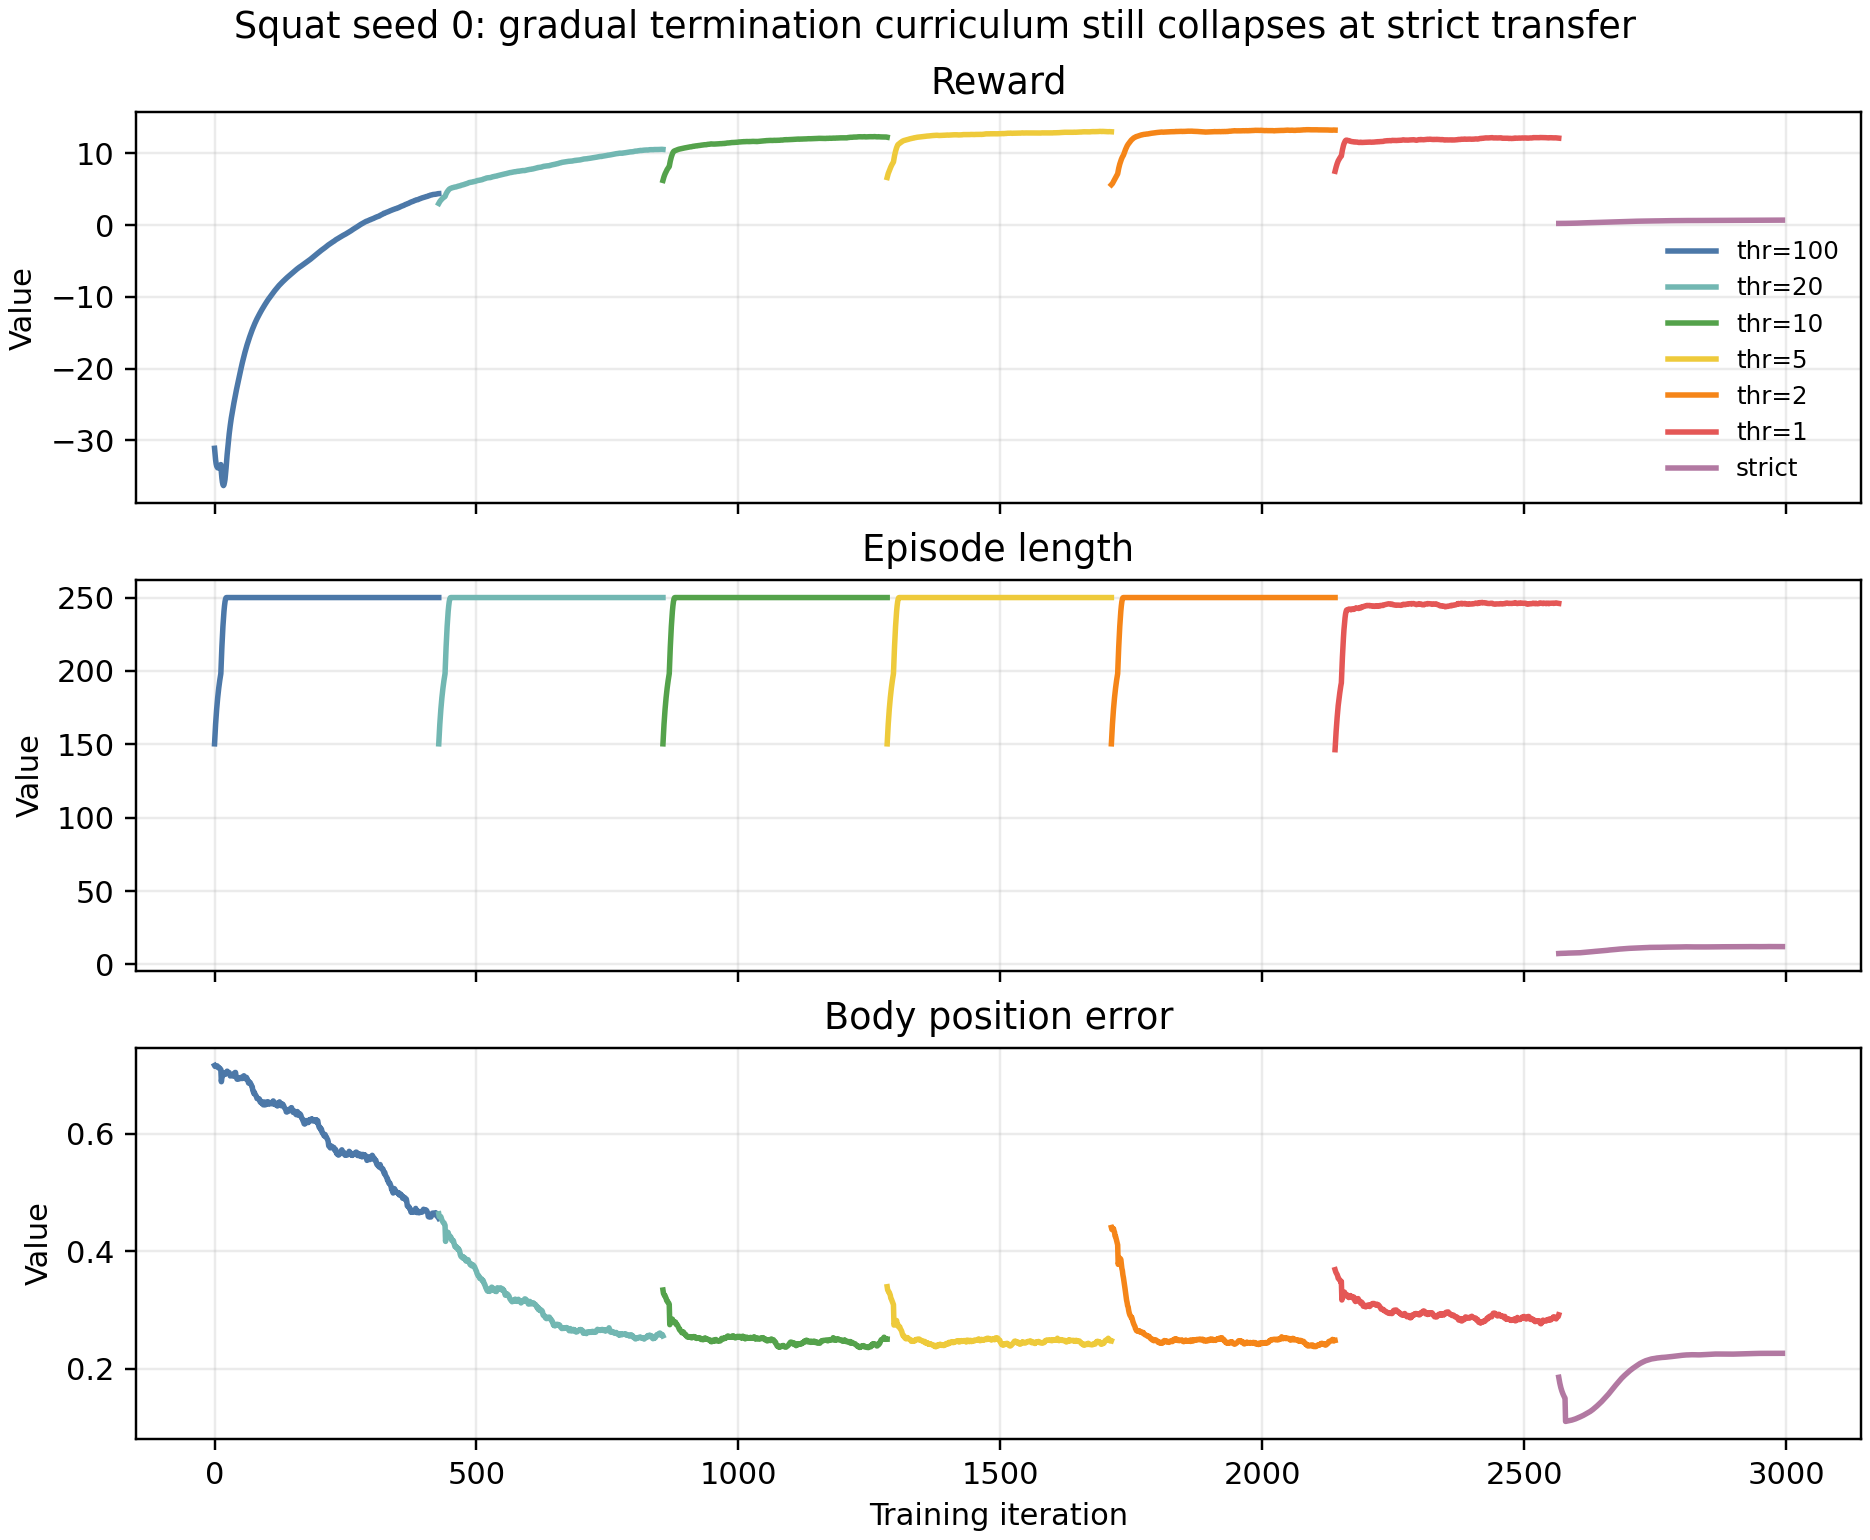
\includegraphics[width=\linewidth]{final_gradual_curriculum_curves.png}
    \caption{Gradual squat curriculum learning curves. Intermediate thresholds preserve long episodes; the final strict stage collapses.}
    \label{fig:gradual_squat}
\end{figure}

\subsection{Direct Calibrated Threshold Training}

The gradual curriculum suggests that the strict seed-0 squat failure is not caused by PPO being unable to learn the generated reference at all. Instead, the failure appears at the termination boundary. We therefore used the gradual-curriculum diagnostic to choose fixed intermediate thresholds and trained new seed-0 squat policies from scratch with thresholds 1 and 2. These runs were interrupted before the planned 2000 iterations, but synchronized logs and videos were preserved through roughly 1200 iterations, which is enough to compare them against the strict failure mode.

Table~\ref{tab:calibrated_threshold} and Figure~\ref{fig:calibrated_threshold} show that calibrated thresholds recover much of the loose-baseline performance without disabling termination entirely. Direct threshold-2 training reaches reward 12.41, full 250-step episodes, and zero final terminations. Direct threshold-1 training is tighter but still mostly recovers, reaching reward 9.21 and 241.82-step episodes with only 0.33 final terminations. In contrast, the default strict seed-0 squat baseline reaches reward 0.84 and only 13.52-step episodes.

\begin{table}[t]
\centering
\caption{Calibrated termination thresholds for seed-0 squat. Direct threshold-2 training recovers full-horizon behavior from scratch, while default strict termination collapses.}
\label{tab:calibrated_threshold}
\resizebox{\linewidth}{!}{
\begin{tabular}{lrrrr}
\toprule
Condition & Reward & Episode length & Body pos. err. & Term. total \\
\midrule
Loose baseline & 13.657 & 250.00 & 0.271 & 0.000 \\
Strict baseline & 0.837 & 13.52 & 0.234 & 144.875 \\
Gradual curriculum, threshold 2 & 13.040 & 250.00 & 0.293 & 0.000 \\
Gradual curriculum, threshold 1 & 11.934 & 244.86 & 0.294 & 0.292 \\
Direct calibrated threshold 2 & 12.405 & 250.00 & 0.263 & 0.000 \\
Direct calibrated threshold 1 & 9.214 & 241.82 & 0.351 & 0.333 \\
\bottomrule
\end{tabular}}
\end{table}

\begin{figure}[t]
    \centering
    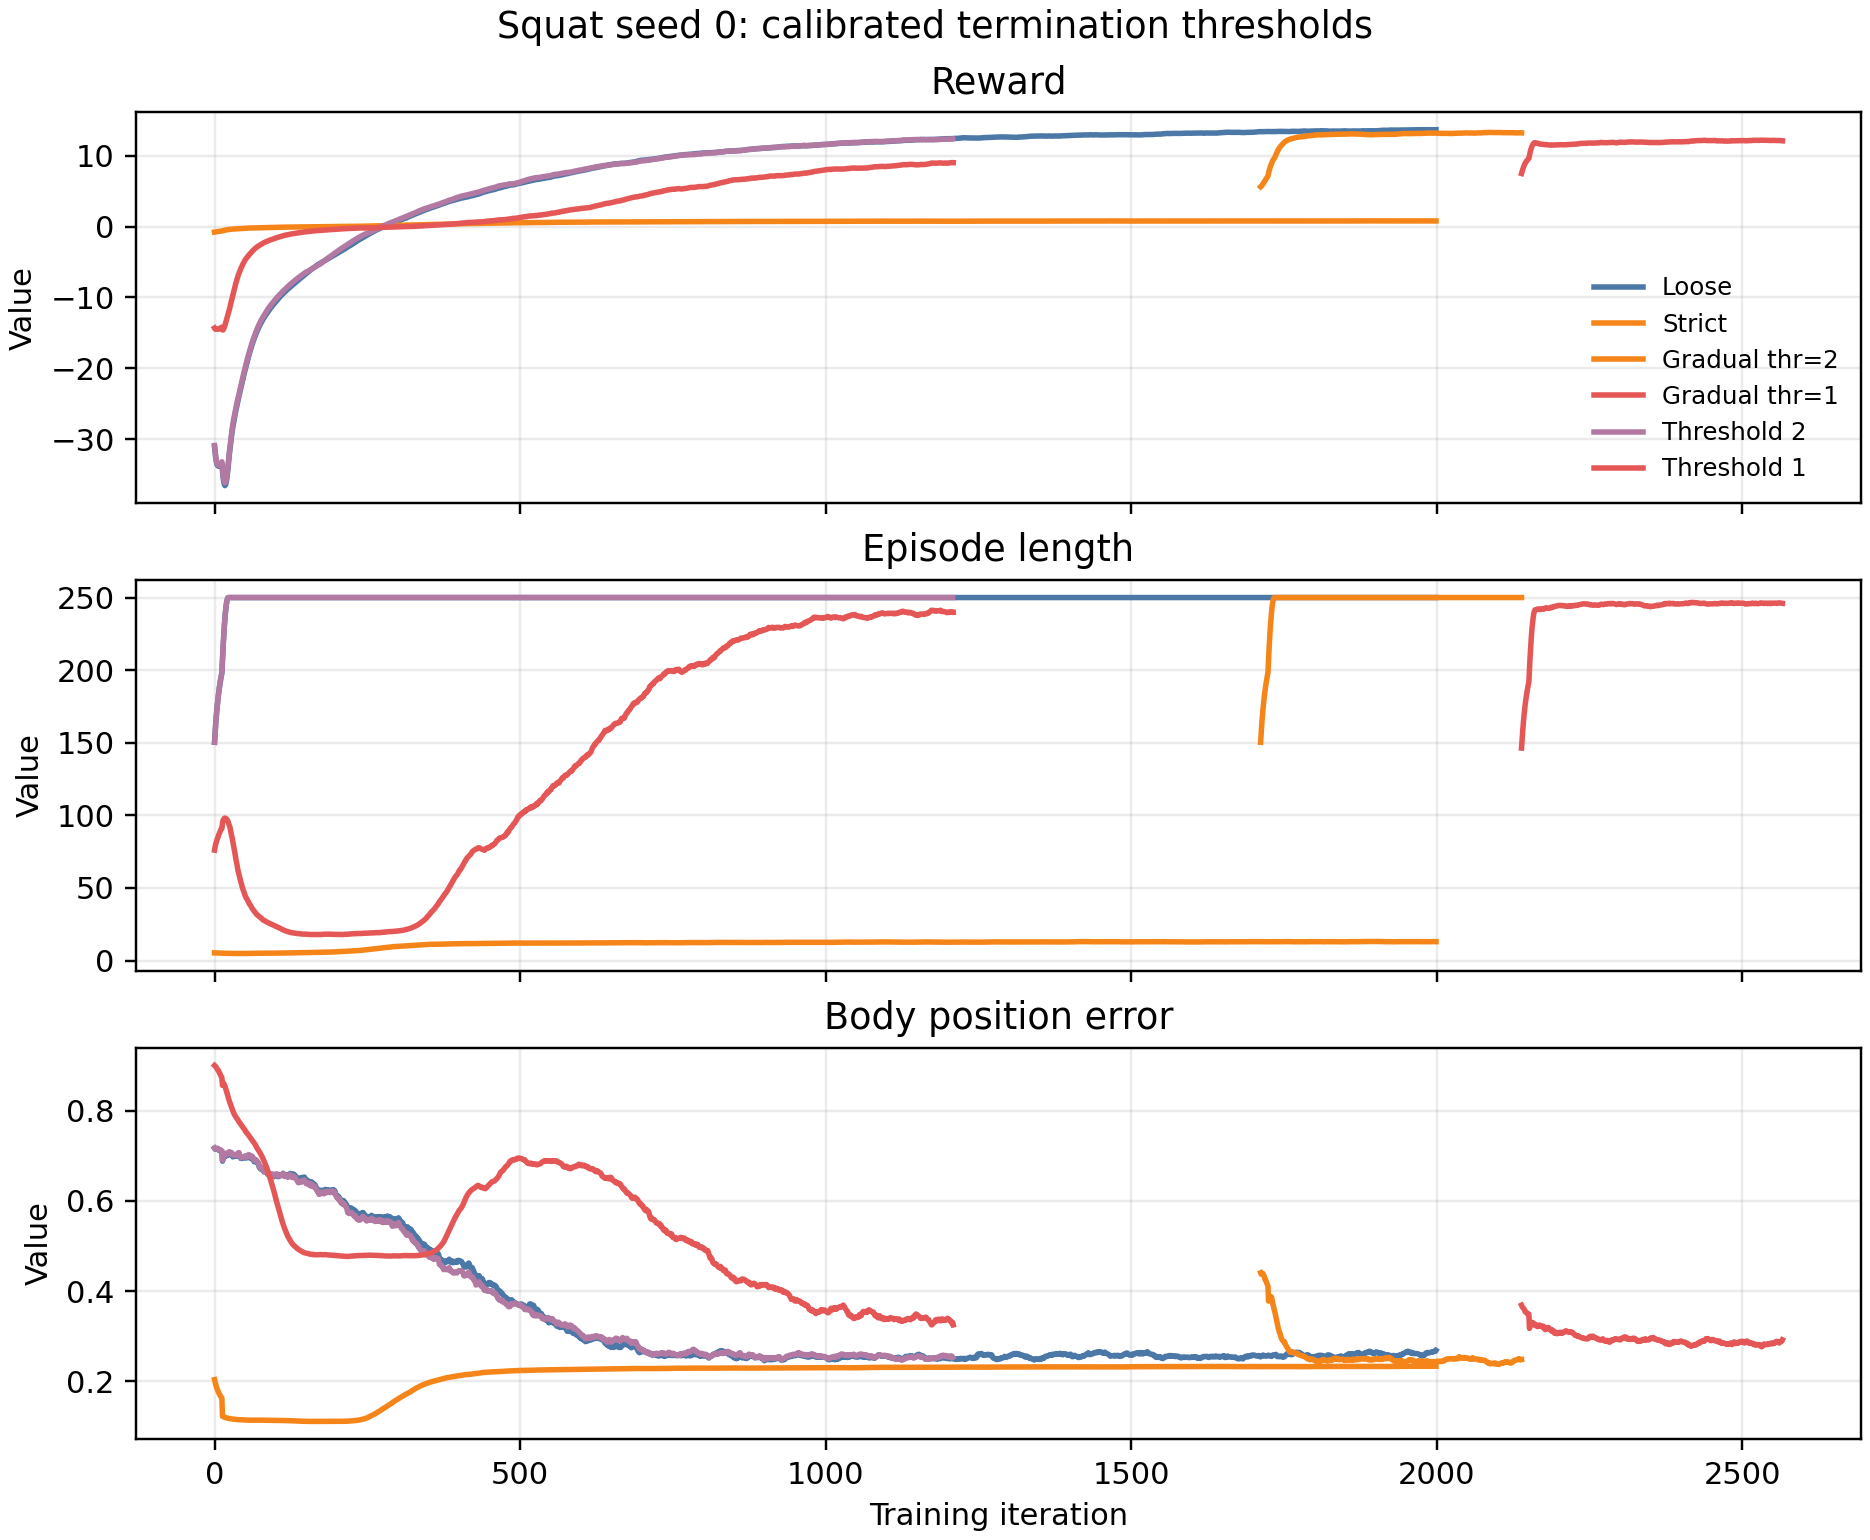
\includegraphics[width=\linewidth]{final_calibrated_threshold_curves.png}
    \caption{Calibrated-threshold squat learning curves. Intermediate thresholds recover long episodes from scratch, unlike the default strict seed-0 baseline.}
    \label{fig:calibrated_threshold}
\end{figure}

\subsection{Jump Training}

We also trained a loose-termination PPO policy for the harder ``a person jumps'' prompt. The run reaches final reward 15.63, full 250-step episodes, body-position error 0.046, joint-position error 0.727, and zero final terminations. This result is useful because it prevents an overly simple story where all semantically harder prompts fail. In this setup, jump is learnable under loose termination, while squat seed 0 remains brittle specifically at the strict termination boundary.

\begin{figure}[t]
    \centering
    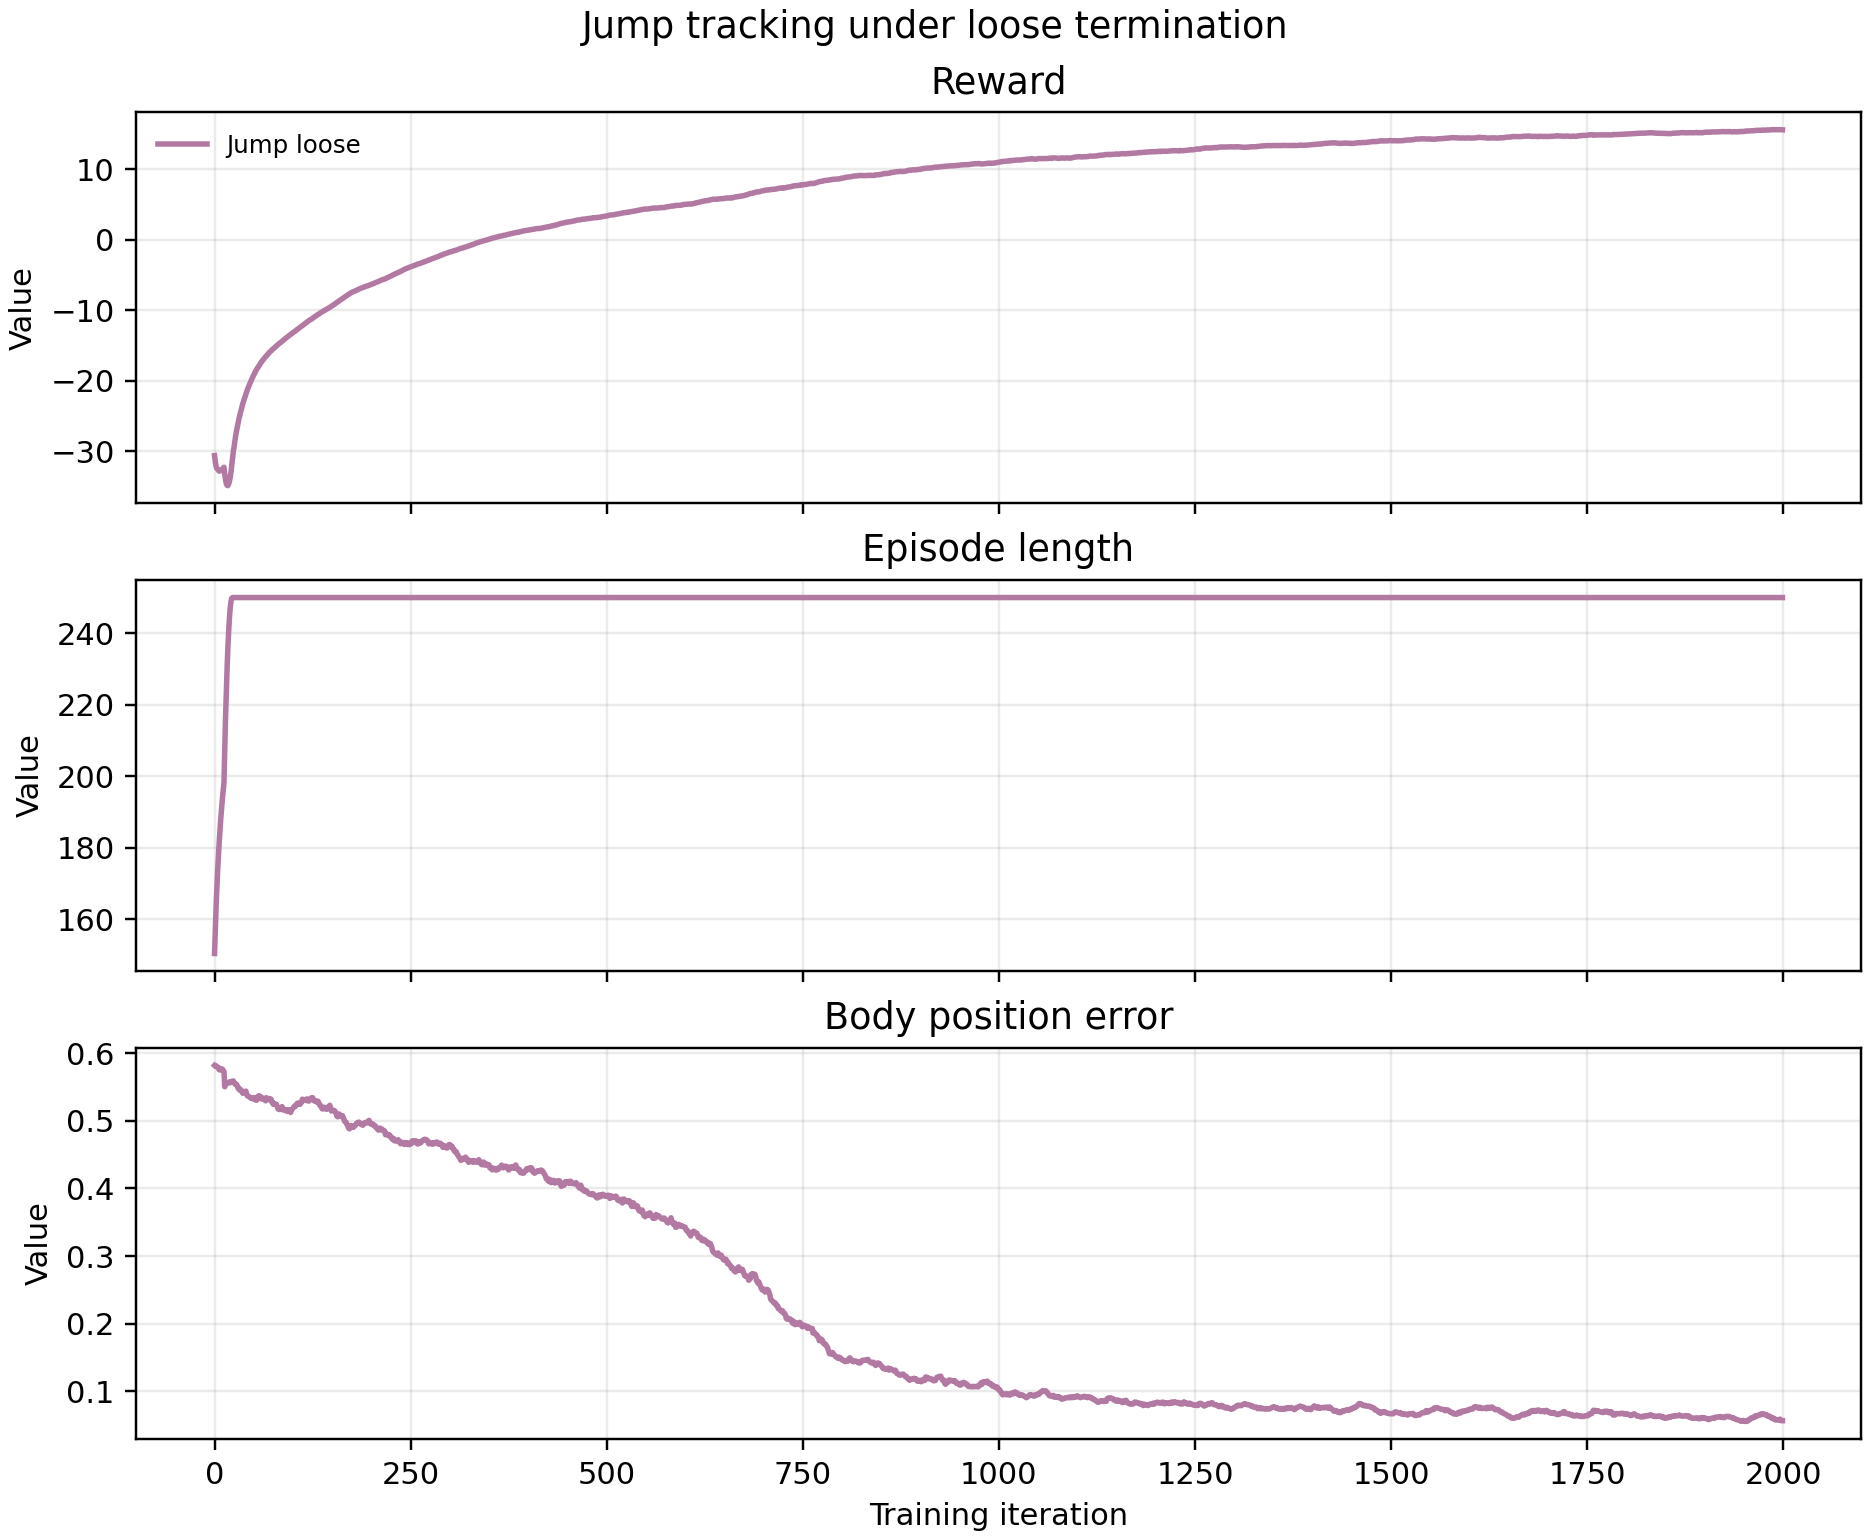
\includegraphics[width=\linewidth]{final_jump_training_curves.png}
    \caption{Loose-termination jump training. The policy reaches full-horizon episodes and stable final reward.}
    \label{fig:jump_curves}
\end{figure}

\subsection{Qualitative Rollouts}

Figures~\ref{fig:squat_sequence}, \ref{fig:gesture_sequence}, \ref{fig:gradual_sequence}, \ref{fig:calibrated_sequence}, and~\ref{fig:jump_sequence} show frame sequences from the saved rollout videos. The qualitative videos match the metrics: strict gesture policies are stable, strict squat repeatedly terminates early, intermediate gradual-curriculum stages produce much longer episodes than the final strict stage, calibrated thresholds recover long squat rollouts, and jump remains stable under loose termination.

\begin{figure}[t]
    \centering
    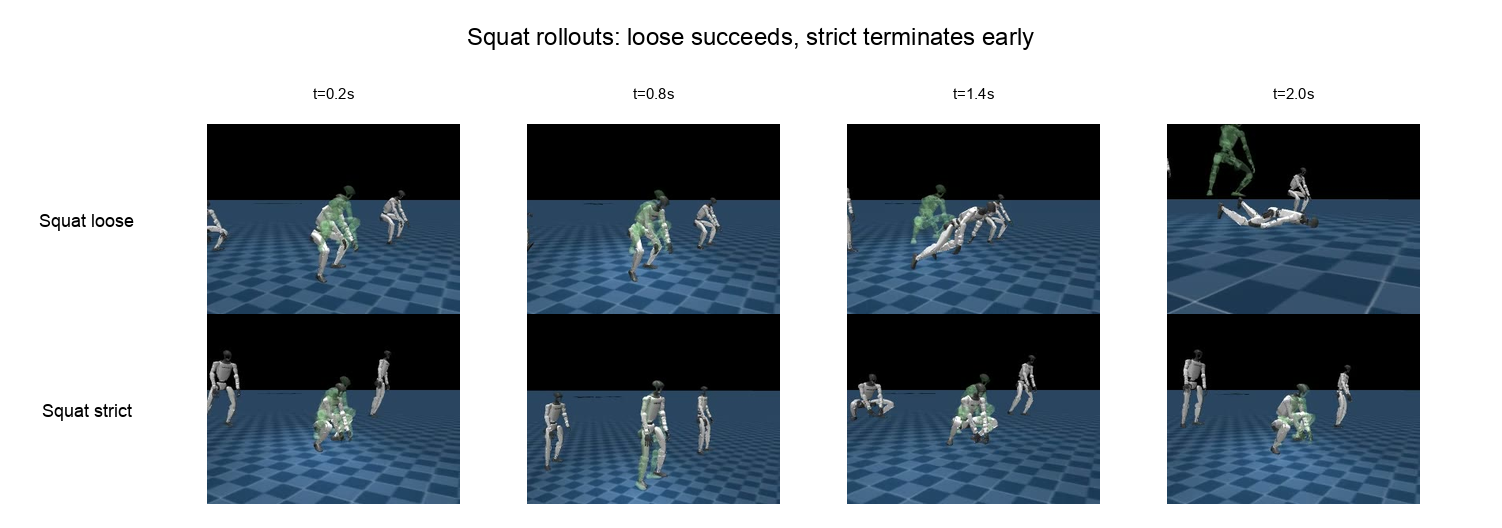
\includegraphics[width=\linewidth]{final_squat_sequence_panel.png}
    \caption{Squat rollout frames at the final checkpoint. Loose training tracks more of the squat reference; strict training terminates early and never learns a full-horizon behavior.}
    \label{fig:squat_sequence}
\end{figure}

\begin{figure}[t]
    \centering
    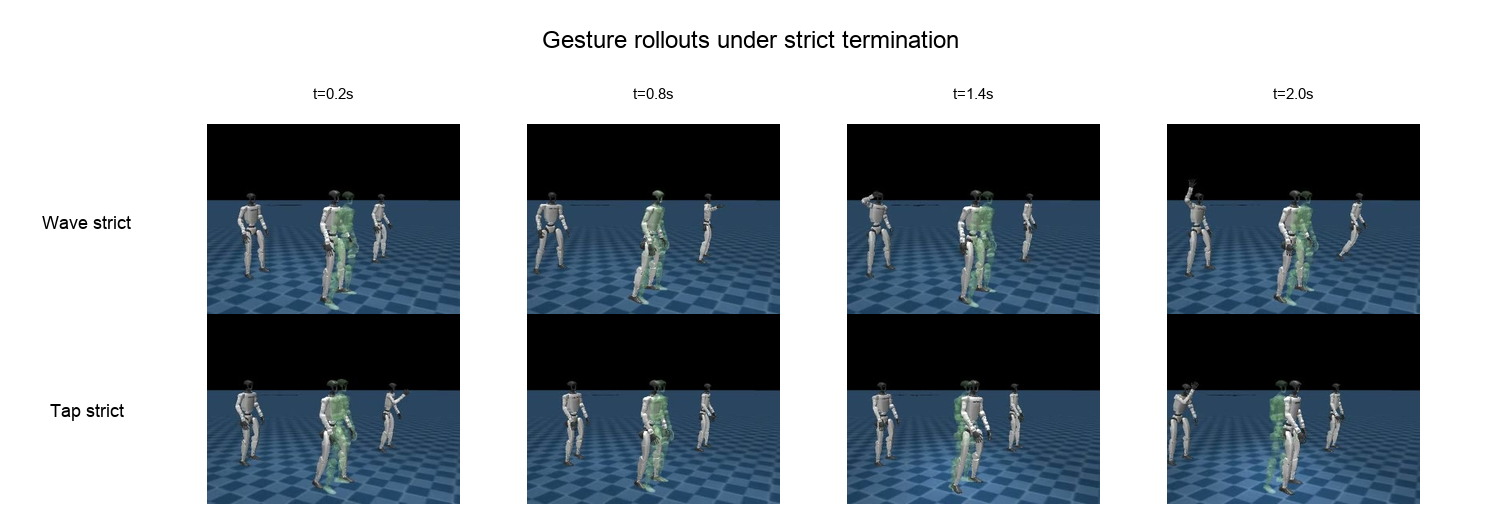
\includegraphics[width=\linewidth]{final_gesture_sequence_panel.png}
    \caption{Gesture rollout frames under strict termination. Wave and tap head remain stable because they do not require large root-height changes.}
    \label{fig:gesture_sequence}
\end{figure}

\begin{figure}[t]
    \centering
    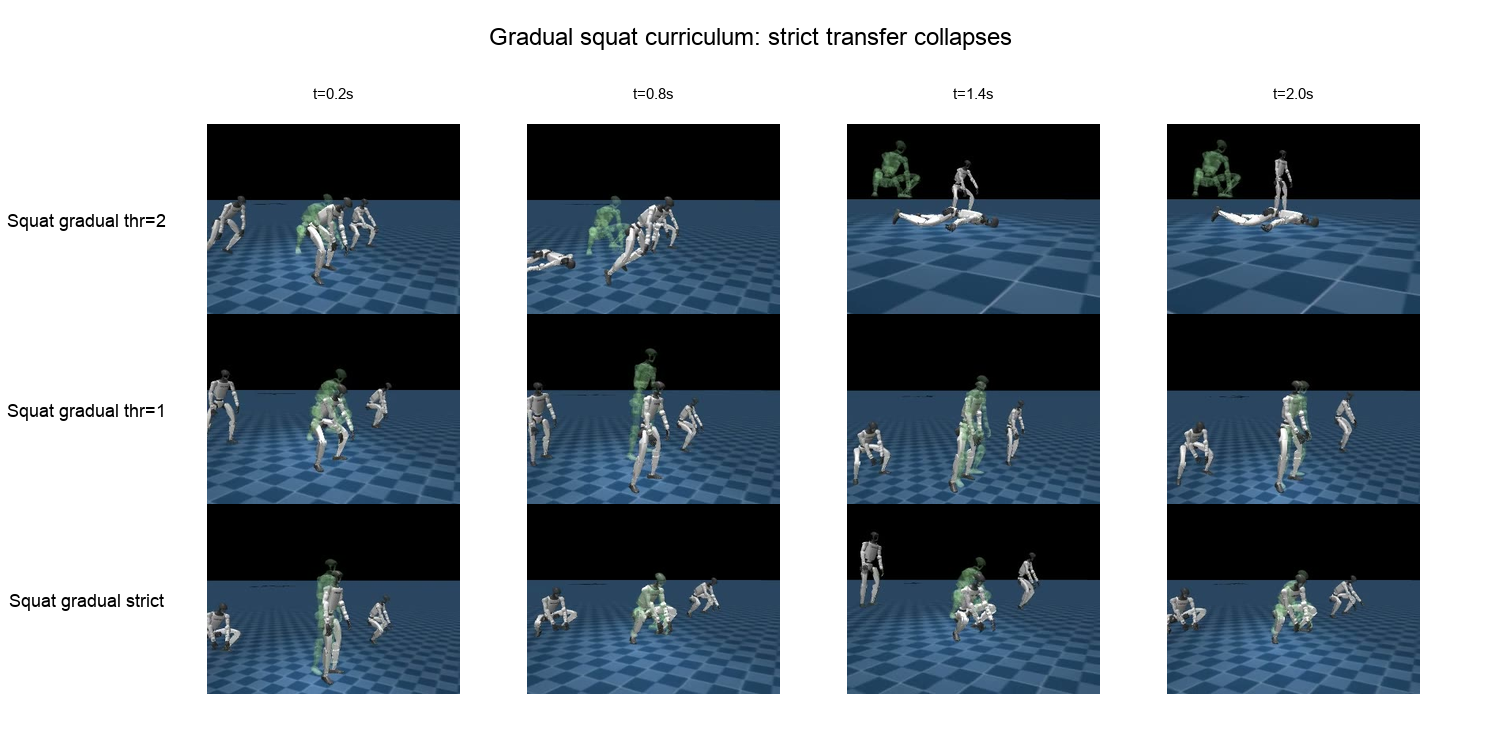
\includegraphics[width=\linewidth]{final_gradual_curriculum_sequence_panel.png}
    \caption{Gradual squat curriculum rollout frames. Intermediate thresholds preserve long episodes in the metrics, while the final strict stage terminates early.}
    \label{fig:gradual_sequence}
\end{figure}

\begin{figure}[t]
    \centering
    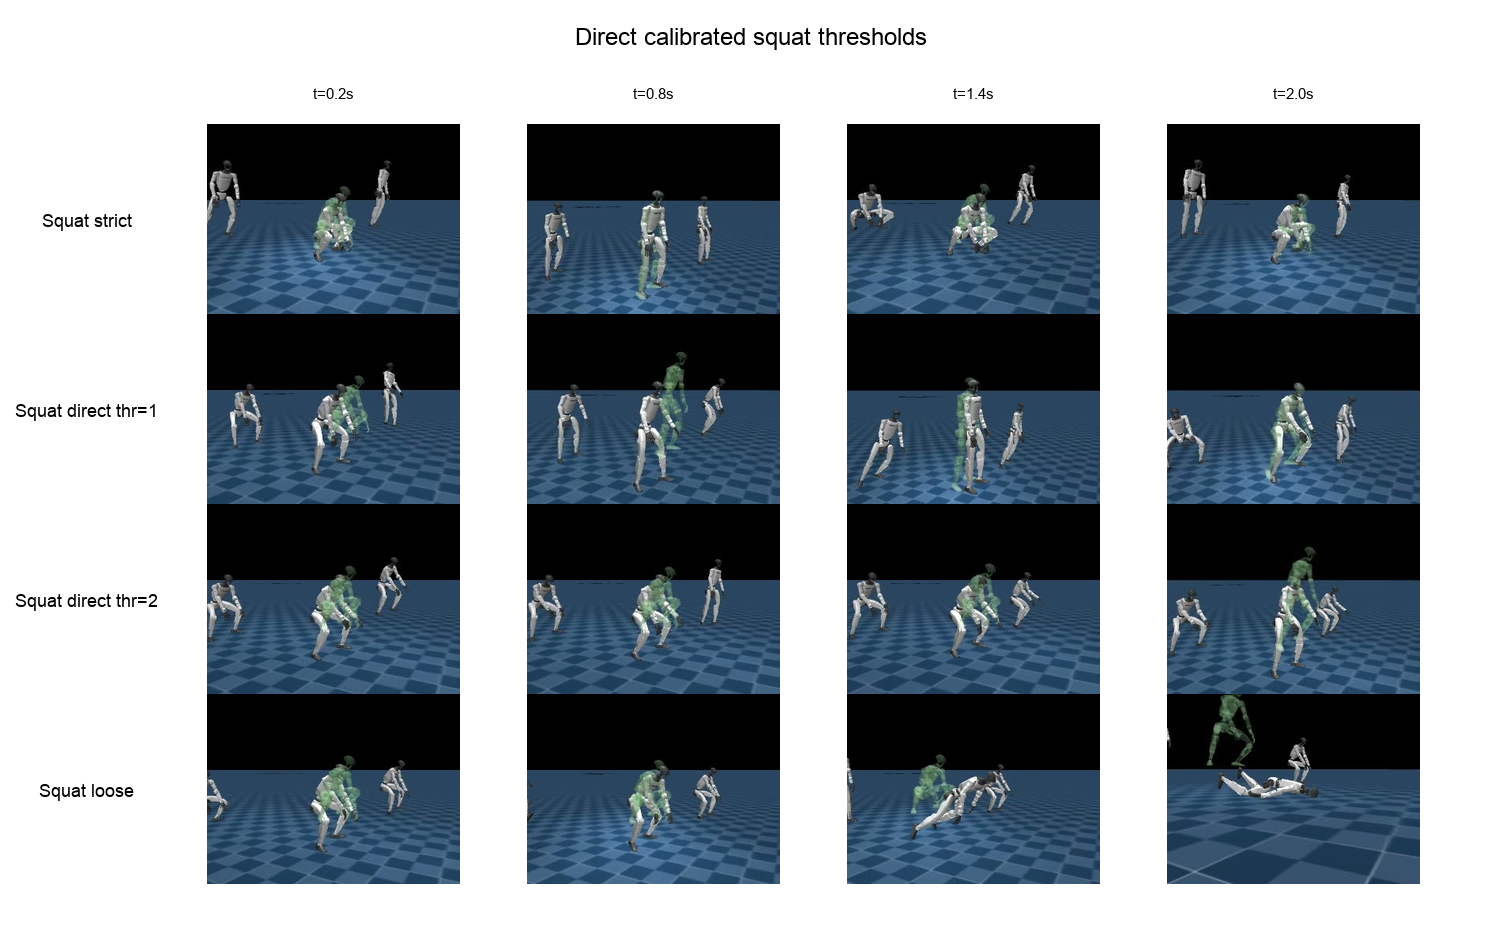
\includegraphics[width=\linewidth]{final_calibrated_threshold_sequence_panel.png}
    \caption{Direct calibrated-threshold squat rollout frames. Thresholds 1 and 2 produce substantially longer rollouts than default strict termination while retaining finite deviation limits.}
    \label{fig:calibrated_sequence}
\end{figure}

\begin{figure}[t]
    \centering
    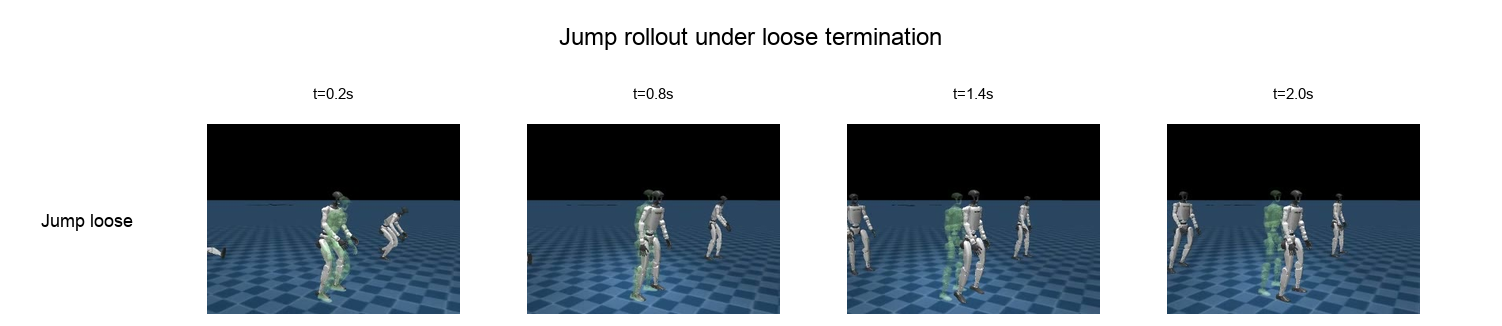
\includegraphics[width=\linewidth]{final_jump_sequence_panel.png}
    \caption{Jump rollout frames after loose-termination PPO training. This harder prompt is learnable under relaxed termination.}
    \label{fig:jump_sequence}
\end{figure}

\subsection{Hard Reference Prompts}

We also generated reference motions for harder prompts: jump, roll forward, backflip, and cartwheel. Figure~\ref{fig:hard_refs} shows that these references are qualitatively useful for diagnosing the generator-controller interface. We trained jump with loose termination, while roll, backflip, and cartwheel remain reference-only. Roll and cartwheel introduce contact-heavy, inverted, or ground-interaction segments, while the backflip prompt does not produce a clean backflip. These references are good candidates for future PPO runs, but the videos alone already show that semantic prompt difficulty and reference feasibility are additional bottlenecks.

\begin{figure}[t]
    \centering
    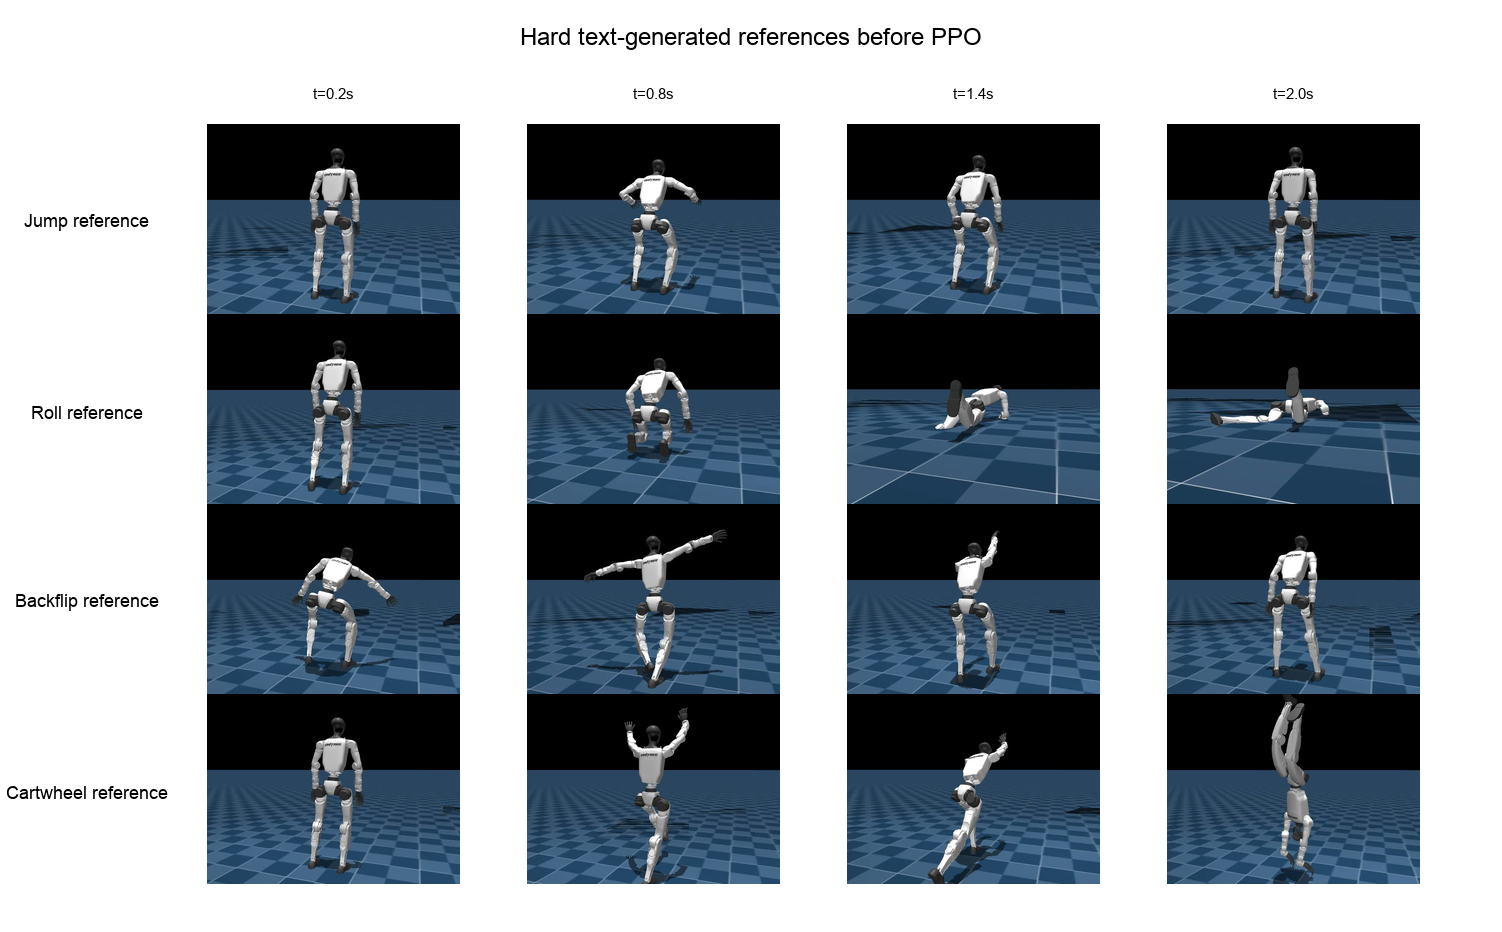
\includegraphics[width=\linewidth]{final_hard_reference_panel.png}
    \caption{Hard prompt references. Jump is later trainable under loose termination, while roll, backflip, and cartwheel expose contact and semantic issues before PPO training is attempted.}
    \label{fig:hard_refs}
\end{figure}

\section{Discussion}

The main lesson is that the generated-motion to physical-control interface is sensitive to termination design, random seed, and training path. Strict terminations are not inherently bad: for static or gesture-heavy references, they preserve stable learning and final tracking quality. For squat, strict termination fails catastrophically on one seed but eventually succeeds on another. Jump also succeeds under loose termination. This suggests that difficult generated references can lie near a learnability boundary where small changes in initialization, generated motion, or exploration history change the outcome.

This also shows why tracking error must be interpreted together with episode length. The strict squat policy has low reported body-position and joint-position error because it only evaluates a short early segment. The more meaningful success indicators are reward, episode length, termination count, and qualitative rollouts.

The curriculum result is negative for final strict performance, but informative. We implemented working loose-to-strict curricula and confirmed that training can resume across stages, but the walk curriculum did not improve over strict training. On squat seed 0, the loose first stage learned a full-horizon policy, but abrupt strict transfer collapsed almost immediately. The gradual schedule survives increasingly strict intermediate thresholds before failing only at the default strict stage. This made it possible to turn the diagnostic into an intervention: training directly with calibrated thresholds 1 or 2 avoids the default strict collapse, with threshold 2 nearly matching the loose baseline while still retaining finite deviation limits. This suggests that a useful curriculum or deployment policy may need explicit threshold calibration, smoother threshold definitions, mixed strict/loose rollouts, or state initialization strategies rather than a single hard switch to default strict thresholds.

\section{Limitations}

This study is intentionally small. Most prompts use one seed, and squat uses two seeds plus additional curriculum runs. The conclusions should be viewed as empirical evidence for a failure mode rather than a broad benchmark. We also use simple diagnostics rather than learned feasibility predictors, and we do not yet estimate foot-contact consistency directly. Roll, backflip, and cartwheel were generated and visualized but not trained with PPO. Finally, all results are in simulation; we do not deploy policies on hardware.

\section{Conclusion}

We built and ran an end-to-end text-to-physics pipeline for Unitree G1 humanoid motion tracking using Kimodo, KimoLab, MuJoCo Warp, and PPO. In our prompt suite, easy gesture references are learnable under strict termination, and a harder jump reference is learnable under loose termination. Squat exposes a more delicate boundary: loose termination succeeds robustly, strict termination fails on one seed but recovers on another, abrupt loose-to-strict curriculum fails on seed 0, and gradual curriculum narrows the failure to the final strict threshold. Using that boundary as an intervention, direct calibrated-threshold training recovers full-horizon squat behavior from scratch. Hard reference-only prompts further show that generated kinematics can be semantically weak or contact-heavy before PPO begins. Overall, the results support the project framing: the key research problem is the failure boundary between text-generated kinematic motion and physically executable humanoid control.

\section*{Team Contributions}

\textbf{Kuzey Kantarcioglu} helped set up and validate the KimoLab/MuJoCo training pipeline, run generated-motion and PPO experiments, inspect training behavior, and interpret failure cases from rollout videos and metrics. Kuzey also contributed to experiment design, prompt selection, and final result analysis.

\textbf{Benji Warburton} helped design the prompt suite and termination-condition experiments, build the Modal orchestration and artifact-download workflow, implement diagnostics and plotting scripts, run PPO experiments on Modal, generate figures and visual assets, and draft the final report.

Both team members contributed to debugging the end-to-end pipeline, selecting final experiments, interpreting the strict-vs-loose termination results, and preparing the poster/report narrative. Compared to the original proposal, more effort shifted toward cloud infrastructure and artifact management than expected because KimoLab/MuJoCo Warp training required GPU containers, Hugging Face gated-model access, periodic checkpoint/video sync, and careful Modal job management.

\section*{AI Tools Disclosure}

We used AI coding assistance to scaffold and revise Modal orchestration scripts, download utilities, diagnostics scripts, plotting scripts, visual asset generation, and report drafting. All reported experiments were run by the team on Modal GPU jobs, and all quantitative results in this report come from saved KimoLab/MuJoCo Warp training logs and generated reference-motion artifacts.

\begin{thebibliography}{9}

\bibitem{kimodo}
D. Rempe et al.
\newblock Kimodo: Scaling Controllable Human Motion Generation.
\newblock NVIDIA Research, 2026.
\newblock \url{https://research.nvidia.com/labs/sil/projects/kimodo}

\bibitem{kimodo_github}
NVIDIA.
\newblock Kimodo official implementation.
\newblock \url{https://github.com/nv-tlabs/kimodo}

\bibitem{kimolab}
Sentdex.
\newblock KimoLab repository.
\newblock \url{https://github.com/Sentdex/kimolab}

\bibitem{mujoco}
E. Todorov, T. Erez, and Y. Tassa.
\newblock MuJoCo: A physics engine for model-based control.
\newblock In \emph{IEEE/RSJ International Conference on Intelligent Robots and Systems}, 2012.

\bibitem{mujocowarp}
Google DeepMind.
\newblock MuJoCo Warp.
\newblock \url{https://github.com/google-deepmind/mujoco_warp}

\bibitem{ppo}
J. Schulman, F. Wolski, P. Dhariwal, A. Radford, and O. Klimov.
\newblock Proximal Policy Optimization Algorithms.
\newblock arXiv:1707.06347, 2017.

\bibitem{deepmimic}
X. B. Peng, P. Abbeel, S. Levine, and M. van de Panne.
\newblock DeepMimic: Example-guided deep reinforcement learning of physics-based character skills.
\newblock \emph{ACM Transactions on Graphics}, 2018.

\bibitem{amp}
X. B. Peng, Z. Ma, P. Abbeel, S. Levine, and A. Kanazawa.
\newblock AMP: Adversarial Motion Priors for stylized physics-based character control.
\newblock \emph{ACM Transactions on Graphics}, 2021.

\end{thebibliography}

\end{document}
